% Template adapted from https://github.com/jgm/pandoc-templates/blob/master/default.latex
% To be used with XeLaTex in memoiR
%%%%%%%%%%%%%%%%%%%%%%%%%%%%%%%%%%%%%%%%%%%%%%%%%%%%%%%%%%%%%%%%%%%%%%%%%%%%%%%%%%%%%%%%%

% Options for packages loaded elsewhere
\PassOptionsToPackage{unicode=true}{hyperref}
\PassOptionsToPackage{hyphens}{url}
\PassOptionsToPackage{dvipsnames,svgnames*,x11names*}{xcolor}
% Right to left support


\documentclass[
  10pt,
  italian,
  a4paper,
  extrafontsizes,onecolumn,openright
  ]{memoir}

% Double (or whatever) spacing

% Math
\usepackage{amssymb, amsmath}
% mathspec: arbitrary math fonts
\usepackage{unicode-math}
\defaultfontfeatures{Scale=MatchLowercase}
\defaultfontfeatures[\rmfamily]{Ligatures=TeX,Scale=1}

% Fonts
\usepackage{lmodern}
\usepackage{fontspec}

% Main font
% Specific sanserif font
% Specific monotype font
\setmonofont[Scale=0.75]{Operator Mono SSm Lig Book}
% Specific math font
% Chinese, Japanese, Corean fonts

% Use upquote for straight quotes in verbatim environments
\usepackage{upquote}
% Use microtype
\usepackage[]{microtype}
\UseMicrotypeSet[protrusion]{basicmath} % disable protrusion for tt fonts

% Verbatim in note

% Color links
\usepackage{xcolor}

% Strikeout

% Necessary for code chunks
\usepackage{color}
\usepackage{fancyvrb}
\newcommand{\VerbBar}{|}
\newcommand{\VERB}{\Verb[commandchars=\\\{\}]}
\DefineVerbatimEnvironment{Highlighting}{Verbatim}{commandchars=\\\{\}}
% Add ',fontsize=\small' for more characters per line
\usepackage{framed}
\definecolor{shadecolor}{RGB}{248,248,248}
\newenvironment{Shaded}{\begin{snugshade}}{\end{snugshade}}
\newcommand{\AlertTok}[1]{\textcolor[rgb]{0.94,0.16,0.16}{#1}}
\newcommand{\AnnotationTok}[1]{\textcolor[rgb]{0.56,0.35,0.01}{\textbf{\textit{#1}}}}
\newcommand{\AttributeTok}[1]{\textcolor[rgb]{0.77,0.63,0.00}{#1}}
\newcommand{\BaseNTok}[1]{\textcolor[rgb]{0.00,0.00,0.81}{#1}}
\newcommand{\BuiltInTok}[1]{#1}
\newcommand{\CharTok}[1]{\textcolor[rgb]{0.31,0.60,0.02}{#1}}
\newcommand{\CommentTok}[1]{\textcolor[rgb]{0.56,0.35,0.01}{\textit{#1}}}
\newcommand{\CommentVarTok}[1]{\textcolor[rgb]{0.56,0.35,0.01}{\textbf{\textit{#1}}}}
\newcommand{\ConstantTok}[1]{\textcolor[rgb]{0.00,0.00,0.00}{#1}}
\newcommand{\ControlFlowTok}[1]{\textcolor[rgb]{0.13,0.29,0.53}{\textbf{#1}}}
\newcommand{\DataTypeTok}[1]{\textcolor[rgb]{0.13,0.29,0.53}{#1}}
\newcommand{\DecValTok}[1]{\textcolor[rgb]{0.00,0.00,0.81}{#1}}
\newcommand{\DocumentationTok}[1]{\textcolor[rgb]{0.56,0.35,0.01}{\textbf{\textit{#1}}}}
\newcommand{\ErrorTok}[1]{\textcolor[rgb]{0.64,0.00,0.00}{\textbf{#1}}}
\newcommand{\ExtensionTok}[1]{#1}
\newcommand{\FloatTok}[1]{\textcolor[rgb]{0.00,0.00,0.81}{#1}}
\newcommand{\FunctionTok}[1]{\textcolor[rgb]{0.00,0.00,0.00}{#1}}
\newcommand{\ImportTok}[1]{#1}
\newcommand{\InformationTok}[1]{\textcolor[rgb]{0.56,0.35,0.01}{\textbf{\textit{#1}}}}
\newcommand{\KeywordTok}[1]{\textcolor[rgb]{0.13,0.29,0.53}{\textbf{#1}}}
\newcommand{\NormalTok}[1]{#1}
\newcommand{\OperatorTok}[1]{\textcolor[rgb]{0.81,0.36,0.00}{\textbf{#1}}}
\newcommand{\OtherTok}[1]{\textcolor[rgb]{0.56,0.35,0.01}{#1}}
\newcommand{\PreprocessorTok}[1]{\textcolor[rgb]{0.56,0.35,0.01}{\textit{#1}}}
\newcommand{\RegionMarkerTok}[1]{#1}
\newcommand{\SpecialCharTok}[1]{\textcolor[rgb]{0.00,0.00,0.00}{#1}}
\newcommand{\SpecialStringTok}[1]{\textcolor[rgb]{0.31,0.60,0.02}{#1}}
\newcommand{\StringTok}[1]{\textcolor[rgb]{0.31,0.60,0.02}{#1}}
\newcommand{\VariableTok}[1]{\textcolor[rgb]{0.00,0.00,0.00}{#1}}
\newcommand{\VerbatimStringTok}[1]{\textcolor[rgb]{0.31,0.60,0.02}{#1}}
\newcommand{\WarningTok}[1]{\textcolor[rgb]{0.56,0.35,0.01}{\textbf{\textit{#1}}}}

% Listings package

% Tables
\usepackage{longtable,booktabs,tabu}
% Fix footnotes in tables (requires footnote package)
\IfFileExists{footnote.sty}{\usepackage{footnote}\makesavenoteenv{longtable}}{}

% Graphics
\usepackage{graphicx,grffile}
\graphicspath{{images/}}
\makeatletter
\def\maxwidth{\ifdim\Gin@nat@width>\linewidth\linewidth\else\Gin@nat@width\fi}
\def\maxheight{\ifdim\Gin@nat@height>\textheight\textheight\else\Gin@nat@height\fi}
\makeatother
% Scale images if necessary, so that they will not overflow the page
% margins by default, and it is still possible to overwrite the defaults
% using explicit options in \includegraphics[width, height, ...]{}
\setkeys{Gin}{width=\maxwidth,height=\maxheight,keepaspectratio}

% Prevent overfull lines
\setlength{\emergencystretch}{3em}  
\providecommand{\tightlist}{%
  \setlength{\itemsep}{0pt}\setlength{\parskip}{0pt}}

% Number sections for memoir (secnumdepth counter is ignored)
\setsecnumdepth{section}

% Set default figure placement to htbp
\makeatletter
\def\fps@figure{htbp}
\makeatother

% Spacing in lists
\usepackage{enumitem}

% Polyglossia
\usepackage{polyglossia}
\setmainlanguage{it}
\setotherlanguage{en-US}

% BibLaTeX
\usepackage[backend=biber,style=authoryear-ibid,isbn=false,backref=true,giveninits=true,uniquename=init,maxcitenames=2,maxbibnames=150,sorting=nyt,sortcites=false,style=apa]{biblatex}
\addbibresource{refs.bib}

% cslreferences environment required by pandoc > 2.7



%%%%%%%%%%%%%%%%%%%%%%%%%%%%%%%%%%%%%%%%%%%%%%%%%%%%%%%%%%
% memoiR format

% Chapter Summary environment 
\usepackage[tikz]{bclogo}
\newenvironment{Summary}
  {\begin{bclogo}[logo=\bctrombone, noborder=true, couleur=lightgray!50]{In breve}\parindent0pt}
  {\end{bclogo}}
% Syntax:
%
%```{block, type='Summary'}
% Deliver message here.
% ```

% scriptsize code 
\let\oldverbatim\verbatim
\def\verbatim{\oldverbatim\scriptsize}
% Applies to code blocks and R code results
% code chunk options size='scriptsize' applies only to R code and results
% if the code chunk sets a different size, \def\verbatim{...} is prioritary for code results 


% Layout
%%%%%%%%%%%%%%%%%%%%%%%%%%%%%%%%%%%%%%%%%%%%%%%%%%%%%%%%%%

% Based on memoir, style companion
\newcommand{\MemoirChapStyle}{daleif1}
\newcommand{\MemoirPageStyle}{Ruled}

% Space between paragraphs
\usepackage{parskip}
  \abnormalparskip{3pt}

% Adjust margin paragraphs vertical position
\usepackage{marginfix}


% Margins
%%%%%%%%%%%%%%%%%%%%%%%%%%%%%%%%%%%%%%%

% allow use of '-',+','/' ans '*' to make simple length computation
\usepackage{calc}

% Full-width figures utilities
\newlength\widthw % full width
\newlength{\rf}
\newcommand*{\definesHSpace}{
  \strictpagecheck % slower but efficient detection of odd/even pages
  \checkoddpage
  \ifoddpage
  \setlength{\rf}{0mm}
  \else
  \setlength{\rf}{\marginparsep+\marginparwidth}
  \fi
}

\makeatletter
% 1" margins for the front matter.
\newcommand*{\SmallMargins}{
  \setlrmarginsandblock{1.5in}{1.5in}{*}
  \setmarginnotes{0.1in}{0.1in}{0.1in}
 \setulmarginsandblock{1.5in}{1in}{*}
  \checkandfixthelayout
  \ch@ngetext
  \clearpage
  \setlength{\widthw}{\textwidth+\marginparsep+\marginparwidth}
  \footnotesatfoot
  \chapterstyle{\MemoirChapStyle}  % Chapter and page styles must be recalled
  \pagestyle{\MemoirPageStyle}
}

% 3" outer margin for the main matter
\newcommand{\LargeMargins}{\SmallMargins}
\makeatother

% Figure captions and footnotes in outer margins


% Main title page with filigrane
%%%%%%%%%%%%%%%%%%%%%%%%%%%%%%%%%%%%%%%%%%%%%%%%%%%%%%%%%%

% Text blocks
\usepackage[absolute,overlay]{textpos}
  \setlength{\TPHorizModule}{1mm}
  \setlength{\TPVertModule}{1mm}

\newcommand{\MainTitlePage}[2]{
  \SmallMargins % Margins
  \pagestyle{empty} % No header/footer
  \textblockorigin{\stockwidth-\paperwidth-\trimedge}{\trimtop} % recto
  \begin{textblock*}{2mm}(\spinemargin/2,\uppermargin/2)
    \rule{1pt}{\paperheight-\uppermargin}
  \end{textblock*}
  \begin{textblock*}{\paperwidth*2/3}(\paperwidth/5, \paperheight/5)
    \flushright
    \begin{Spacing}{3}
      {\fontfamily{qtm}\selectfont\fontsize{45}{45}\selectfont\textsc{\thetitle}}
    \end{Spacing}
  \end{textblock*}
    \begin{textblock*}{\paperwidth*2/3}(\paperwidth/5, \paperheight/2)
    \flushright
    {\fontfamily{qtm}\huge\theauthor}
  \end{textblock*}
    \begin{textblock*}{\paperwidth*2/3}[0, 1](\spinemargin, \uppermargin+\textheight)
    \normalfont\thedate
  \end{textblock*}
  ~\\ % Print a character or the page will not exist
  \newpage
  \textblockorigin{\trimedge}{\trimtop} % verso
  \begin{textblock*}{\textwidth}(\paperwidth-\spinemargin-\textwidth, \uppermargin)
    #1
  \end{textblock*}
  \begin{textblock*}{\textwidth}[0,1](\paperwidth-\spinemargin-\textwidth, \uppermargin+\textheight+\footskip)
    \centering
    
\includegraphics[width=\paperwidth/4]{logo}\\ \bigskip
    #2
  \end{textblock*}
  ~\\ % Print a character or the page will not exist
  \newpage
}

% Clear page and open an even one (\clearpage opens an odd one)
\newcommand{\evenpage}{
  \clearpage
  \strictpagecheck % slower but efficient detection of odd/even pages
  \checkoddpage
  \ifoddpage
    \thispagestyle{empty}
    ~\\ % Print a character or the page will not exist
    \newpage
  \else
    % do nothing
  \fi
}


%% PDF title page to insert
%%%%%%%%%%%%%%%%%%%%%%%%%%%%%%%%%%%%%%%%%%%%%%%%%%%%%%%%%%



%% Bibliography
%%%%%%%%%%%%%%%%%%%%%%%%%%%%%%%%%%%%%%%%%%%%%%%%%%%%%%%%%%

\usepackage[strict,autostyle]{csquotes}
% Repeated citation as author-year-title instead of author-title (modification of footcite:note in verbose-inote.cbx)

%% Table of Contents
%%%%%%%%%%%%%%%%%%%%%%%%%%%%%%%%%%%%%%%%%%%%%%%%%%%%%%%%%%

% fix the typesetting of the part number
\renewcommand\partnumberlinebox[2]{#2\ ---\ }


% Fonts
%%%%%%%%%%%%%%%%%%%%%%%%%%%%%%%%%%%%%%%%%%%%%%%%%%%%%%%%%%


% Hyperref comes last
%%%%%%%%%%%%%%%%%%%%%%%%%%%%%%%%%%%%%%%%%%%%%%%%%%%%%%%%%%

\usepackage{hyperref}
\hypersetup{
  pdftitle={Psicometria},
  pdfauthor={Corrado Caudek},
  colorlinks=true,
  linkcolor=Maroon,
  citecolor=Blue,
  urlcolor=Blue,
  breaklinks=true}

% Don't use monospace font for urls
\urlstyle{same}


% Title, author, date from YAML to LaTeX
%%%%%%%%%%%%%%%%%%%%%%%%%%%%%%%%%%%%%%%%%%%%%%%%%%%%%%%%%%

\title{Psicometria}

\author{Corrado Caudek}

\date{2021-12-03}


% Include headers (preamble.tex) here
%%%%%%%%%%%%%%%%%%%%%%%%%%%%%%%%%%%%%%%%%%%%%%%%%%%%%%%%%%
% Add LaTeX code into the preamble of the document here
\hyphenation{bio-di-ver-si-ty sap-lings}


%%%%%%%%%%%%%%%%%%%%%%%%%%%%%%%%%%%%%%%%%%%%%%%%%%%%%%%%%%%%%%%%%%%%%%%%%
% memoiR dalef3 chapter style 
% https://ctan.crest.fr/tex-archive/info/latex-samples/MemoirChapStyles/MemoirChapStyles.pdf
\usepackage{soul}
\definecolor{nicered}{rgb}{.647,.129,.149}
\makeatletter
\newlength\dlf@normtxtw
\setlength\dlf@normtxtw{\textwidth}
\def\myhelvetfont{\def\sfdefault{mdput}}
\newsavebox{\feline@chapter}
\newcommand\feline@chapter@marker[1][4cm]{%
  \sbox\feline@chapter{%
    \resizebox{!}{#1}{\fboxsep=1pt%
	  \colorbox{nicered}{\color{white}\bfseries\sffamily\thechapter}%
	}}%
  \rotatebox{90}{%
    \resizebox{%
	  \heightof{\usebox{\feline@chapter}}+\depthof{\usebox{\feline@chapter}}}%
	{!}{\scshape\so\@chapapp}}\quad%
  \raisebox{\depthof{\usebox{\feline@chapter}}}{\usebox{\feline@chapter}}%
 }
\newcommand\feline@chm[1][4cm]{%
  \sbox\feline@chapter{\feline@chapter@marker[#1]}%
  \makebox[0pt][l]{% aka \rlap
    \makebox[1cm][r]{\usebox\feline@chapter}%
  }}
\makechapterstyle{daleif1}{
  \renewcommand\chapnamefont{\normalfont\Large\scshape\raggedleft\so}
  \renewcommand\chaptitlefont{\normalfont\huge\bfseries\scshape\color{nicered}}
  \renewcommand\chapternamenum{}
  \renewcommand\printchaptername{}
  \renewcommand\printchapternum{\null\hfill\feline@chm[2.5cm]\par}
  \renewcommand\afterchapternum{\par\vskip\midchapskip}
  \renewcommand\printchaptertitle[1]{\chaptitlefont\raggedleft ##1\par}
}
\makeatother

\DeclareMathOperator{\Var}{Var} % Define variance operator
\DeclareMathOperator{\SD}{SD} % Define sd operator
\DeclareMathOperator{\Cov}{Cov} % Define covariance operator
\DeclareMathOperator{\Corr}{Corr} % Define correlation operator
\DeclareMathOperator{\Me}{Me} % Define mediane operator
\DeclareMathOperator{\Mo}{Mo} % Define mode operator
\DeclareMathOperator{\Bin}{Bin} % Define binomial operator
\DeclareMathOperator{\Bernoulli}{Bernoulli} % Define Bernoulli operator
\DeclareMathOperator{\Poi}{Poi} % Define Poisson operator
\DeclareMathOperator{\Uniform}{Uniform} % Define Uniform operator
\DeclareMathOperator{\Cauchy}{Cauchy} % Define Cauchy operator
\DeclareMathOperator{\elpd}{elpd} % Define elpd operator
\DeclareMathOperator{\lppd}{lppd} % Define lppd operator
\DeclareMathOperator{\LOO}{LOO} % Define LOO operator
\DeclareMathOperator{\B}{\mathscr{B}} % Define Bernoulli operator
\newcommand{\R}{\textsf{R}} % Define R programming language symbol
\newcommand{\E}{\mathbb{E}} % Define expected value operator
\newcommand{\Real}{\mathbb{R}} % Define real number operator
\newcommand{\Prob}{\mathscr{P}}
\DeclareMathOperator*{\argmin}{arg\,min} % thin space, limits on side in displays
\DeclareMathOperator*{\argmax}{arg\,max} % thin space, limits on side in displays

\raggedbottom % allow variable (ragged) site heights
\frenchspacing

\usepackage[
  labelfont=bf, 
  font={small, it} 
]{caption} 
\usepackage{upquote} % print correct quotes in verbatim-environments
\usepackage{empheq} 
\usepackage{xfrac}




\usepackage{booktabs}
\usepackage{longtable}
\usepackage{array}
\usepackage{multirow}
\usepackage{wrapfig}
\usepackage{float}
\usepackage{colortbl}
\usepackage{pdflscape}
\usepackage{tabu}
\usepackage{threeparttable}
\usepackage{threeparttablex}
\usepackage[normalem]{ulem}
\usepackage{makecell}
\usepackage{xcolor}


% End of preamble
%%%%%%%%%%%%%%%%%%%%%%%%%%%%%%%%%%%%%%%%%%%%%%%%%%%%%%%%%%


\usepackage{amsthm}
\newtheorem{theorem}{Teorema}[chapter]
\newtheorem{lemma}{Lemma}[chapter]
\newtheorem{corollary}{Corollario}[chapter]
\newtheorem{proposition}{Proposizione}[chapter]
\newtheorem{conjecture}{Congettura}[chapter]
\theoremstyle{definition}
\newtheorem{definition}{Definizione}[chapter]
\theoremstyle{definition}
\newtheorem{example}{Esempio}[chapter]
\theoremstyle{definition}
\newtheorem{exercise}{Exercizio}[chapter]
\theoremstyle{definition}
\newtheorem{hypothesis}{Hypothesis}[chapter]
\theoremstyle{remark}
\newtheorem*{remark}{Osservazione}
\newtheorem*{solution}{Soluzione}
\begin{document}
\frontmatter

% Title page
%%%%%%%%%%%%%%%%%%%%%%%%%%%%%%%%%%%%%%%%%%%%%%%%%%%%%%%%%%


\MainTitlePage{Questo documento è stato realizzato con:

\begin{itemize}
  \item \LaTeX\; e la classe memoir (\url{http://www.ctan.org/pkg/memoir});
  \item $\R$ (\url{http://www.r-project.org/}) e RStudio (\url{http://www.rstudio.com/});
  \item bookdown (\url{http://bookdown.org/}) e memoiR (\url{https://ericmarcon.github.io/memoiR/}).
\end{itemize}}{Nel blog della mia pagina personale sono forniti alcuni approfondimenti degli argomenti qui trattati.

\url{https://ccaudek.github.io/caudeklab/}}


% Before Body
%%%%%%%%%%%%%%%%%%%%%%%%%%%%%%%%%%%%%%%%%%%%%%%%%%%%%%%%%%





% Contents
%%%%%%%%%%%%%%%%%%%%%%%%%%%%%%%%%%%%%%%%%%%%%%%%%%%%%%%%%%

\LargeMargins
{
\hypersetup{linkcolor=}
\setcounter{tocdepth}{2}
\tableofcontents
}


% Body
%%%%%%%%%%%%%%%%%%%%%%%%%%%%%%%%%%%%%%%%%%%%%%%%%%%%%%%%%%

\LargeMargins
\scriptsize

\normalsize

\chapter*{}

\vfill

\scriptsize

\normalsize

\scriptsize

Copyright \(\copyright\) 2022.

\normalsize

Data della versione presente: Dicembre 03, 2021.

\hypertarget{prefazione}{%
\chapter{Prefazione}\label{prefazione}}

\textbf{Data Science per psicologi} contiene il materiale delle lezioni dell'insegnamento di \emph{Psicometria B000286} (A.A. 2021/2022) rivolto agli studenti del primo anno del Corso di Laurea in Scienze e Tecniche Psicologiche dell'Università degli Studi di Firenze.

L'insegnamento di Psicometria si propone di fornire agli studenti un'introduzione all'analisi dei dati in psicologia.
Le conoscenze/competenze che verranno sviluppate in questo insegnamento sono quelle della \emph{Data science}, ovvero le conoscenze/competenze che si pongono all'intersezione tra statistica (ovvero, richiedono la capacità di comprendere teoremi statistici) e informatica (ovvero, richiedono la capacità di sapere utilizzare un software).

\hypertarget{la-psicologia-e-la-data-science}{%
\section*{La psicologia e la Data Science}\label{la-psicologia-e-la-data-science}}
\addcontentsline{toc}{section}{La psicologia e la Data Science}

\begin{quote}
It's worth noting, before getting started, that this material is hard. If you find yourself confused at any point, you are normal. Any sense of confusion you feel is just your brain correctly calibrating to the subject matter. Over time, confusion is replaced by comprehension {[}\ldots{]} --- Richard McElreath
\end{quote}

Sembra sensato spendere due parole su un tema che è importante per gli studenti: quello indicato dal titolo di questo Capitolo. È ovvio che agli studenti di psicologia la statistica non piace. Se piacesse, forse studierebbero Data Science e non psicologia; ma non lo fanno. Di conseguenza, gli studenti di psicologia si chiedono: ``perché dobbiamo perdere tanto tempo a studiare queste cose quando in realtà quello che ci interessa è tutt'altro?'\,' Questa è una bella domanda.

C'è una ragione molto semplice che dovrebbe farci capire perché la Data Science è così importante per la psicologia. Infatti, a ben pensarci, la psicologia è una disciplina intrinsecamente statistica, se per statistica intendiamo quella disciplina che studia la variazione delle caratteristiche degli individui nella popolazione. La psicologia studia \emph{gli individui} ed è proprio la variabilità inter- e intra-individuale ciò che vogliamo descrivere e, in certi casi, predire. In questo senso, la psicologia è molto diversa dall'ingegneria, per esempio. Le proprietà di un determinato ponte sotto certe condizioni, ad esempio, sono molto simili a quelle di un altro ponte, sotto le medesime condizioni. Quindi, per un ingegnere la statistica è poco importante: le proprietà dei materiali sono unicamente dipendenti dalla loro composizione e restano costanti. Ma lo stesso non può dirsi degli individui: ogni individuo è unico e cambia nel tempo. E le variazioni tra gli individui, e di un individuo nel tempo, sono l'oggetto di studio proprio della psicologia: è dunque chiaro che i problemi che la psicologia si pone sono molto diversi da quelli affrontati, per esempio, dagli ingegneri. Questa è la ragione per cui abbiamo tanto bisogno della \emph{data science} in psicologia: perché la \emph{data science} ci consente di descrivere la variazione e il cambiamento. E queste sono appunto le caratteristiche di base dei fenomeni psicologici.

Sono sicuro che, leggendo queste righe, a molti studenti sarà venuta in mente la seguente domanda: perché non chiediamo a qualche esperto di fare il ``lavoro sporco'' (ovvero le analisi statistiche) per noi, mentre noi (gli psicologi) ci occupiamo solo di ciò che ci interessa, ovvero dei problemi psicologici slegati dai dettagli ``tecnici'' della \emph{data science}?
La risposta a questa domanda è che non è possibile progettare uno studio psicologico sensato senza avere almeno una comprensione rudimentale della \emph{data science}. Le tematiche della \emph{data science} non possono essere ignorate né dai ricercatori in psicologia né da coloro che svolgono la professione di psicologo al di fuori dell'Università. Infatti, anche i professionisti al di fuori dall'università non possono fare a meno di leggere la letteratura psicologica più recente: il continuo aggiornamento delle conoscenze è infatti richiesto dalla deontologia della professione. Ma per potere fare questo è necessario conoscere un bel po' di \emph{data science}! Basta aprire a caso una rivista specialistica di psicologia per rendersi conto di quanto ciò sia vero: gli articoli che riportano i risultati delle ricerche psicologiche sono zeppi di analisi statistiche e di modelli formali. E la comprensione della letteratura psicologica rappresenta un requisito minimo nel bagaglio professionale dello psicologo.

Le considerazioni precedenti cercano di chiarire il seguente punto: la \emph{data science} non è qualcosa da studiare a malincuore, in un singolo insegnamento universitario, per poi poterla tranquillamente dimenticare. Nel bene e nel male, gli psicologi usano gli strumenti della \emph{data science} in tantissimi ambiti della loro attività professionale: in particolare quando costruiscono, somministrano e interpretano i test psicometrici. È dunque chiaro che possedere delle solide basi di \emph{data science} è un tassello imprescindibile del bagaglio professionale dello psicologo. In questo insegnamento verrano trattati i temi base della \emph{data science} e verrà adottato un punto di vista bayesiano, che corrisponde all'approccio più recente e sempre più diffuso in psicologia.

\hypertarget{come-studiare}{%
\section*{Come studiare}\label{come-studiare}}
\addcontentsline{toc}{section}{Come studiare}

\begin{quote}
I know quite certainly that I myself have no special talent. Curiosity, obsession and dogged endurance, combined with self-criticism, have brought me to my ideas. --- Albert Einstein
\end{quote}

Il giusto metodo di studio per prepararsi all'esame di Psicometria è quello di seguire attivamente le lezioni, assimilare i concetti via via che essi vengono presentati e verificare in autonomia le procedure presentate a lezione. Incoraggio gli studenti a farmi domande per chiarire ciò che non è stato capito appieno. Incoraggio gli studenti a utilizzare i forum attivi su Moodle e, soprattutto, a svolgere gli esercizi proposti su Moodle. I problemi forniti su Moodle rappresentano il livello di difficoltà richiesto per superare l'esame e consentono allo studente di comprendere se le competenze sviluppate fino a quel punto sono sufficienti rispetto alle richieste dell'esame.

La prima fase dello studio, che è sicuramente individuale, è quella in cui è necessario acquisire le conoscenze teoriche relative ai problemi che saranno presentati all'esame. La seconda fase di studio, che può essere facilitata da scambi con altri e da incontri di gruppo, porta ad acquisire la capacità di applicare le conoscenze: è necessario capire come usare un software (\R) per applicare i concetti statistici alla specifica situazione del problema che si vuole risolvere. Le due fasi non sono però separate: il saper fare molto spesso ci aiuta a capire meglio.

\hypertarget{sviluppare-un-metodo-di-studio-efficace}{%
\section*{Sviluppare un metodo di studio efficace}\label{sviluppare-un-metodo-di-studio-efficace}}
\addcontentsline{toc}{section}{Sviluppare un metodo di studio efficace}

\begin{quote}
Memorization is not learning. --- Richard Phillips Feynman
\end{quote}

Avendo insegnato molte volte in passato un corso introduttivo di analisi dei dati ho notato nel corso degli anni che gli studenti con l'atteggiamento mentale che descriverò qui sotto generalmente ottengono ottimi risultati. Alcuni studenti sviluppano naturalmente questo approccio allo studio, ma altri hanno bisogno di fare uno sforzo per maturarlo. Fornisco qui sotto una breve descrizione del ``metodo di studio'\,' che, nella mia esperienza, è il più efficace per affrontare le richieste di questo insegnamento \autocite{burger20125}.

\begin{itemize}
\tightlist
\item
  Dedicate un tempo sufficiente al materiale di base, apparentemente facile; assicuratevi di averlo capito bene. Cercate le lacune nella vostra comprensione. Leggere presentazioni diverse dello stesso materiale (in libri o articoli diversi) può fornire nuove intuizioni.
\end{itemize}

\begin{itemize}
\item
  Gli errori che facciamo sono i nostri migliori maestri. Istintivamente cerchiamo di dimenticare subito i nostri errori. Ma il miglior modo di imparare è apprendere dagli errori che commettiamo. In questo senso, una soluzione corretta è meno utile di una soluzione sbagliata. Quando commettiamo un errore questo ci fornisce un'informazione importante: ci fa capire qual è il materiale di studio sul quale dobbiamo ritornare e che dobbiamo capire meglio.
\item
  C'è ovviamente un aspetto ``psicologico'' nello studio. Quando un esercizio o problema ci sembra incomprensibile, la cosa migliore da fare è dire: ``mi arrendo'', ``non ho idea di cosa fare!''. Questo ci rilassa: ci siamo già arresi, quindi non abbiamo niente da perdere, non dobbiamo più preoccuparci. Ma non dobbiamo fermarci qui. Le cose ``migliori'' che faccio (se ci sono) le faccio quando non ho voglia di lavorare. Alle volte, quando c'è qualcosa che non so fare e non ho idea di come affontare, mi dico: ``oggi non ho proprio voglia di fare fatica'', non ho voglia di mettermi nello stato mentale per cui ``in 10 minuti devo risolvere il problema perché dopo devo fare altre cose''. Però ho voglia di \emph{divertirmi} con quel problema e allora mi dedico a qualche aspetto ``marginale'' del problema, che so come affrontare, oppure considero l'aspetto più difficile del problema, quello che non so come risolvere, ma invece di cercare di risolverlo, guardo come altre persone hanno affrontato problemi simili, opppure lo stesso problema in un altro contesto. Non mi pongo l'obiettivo ``risolvi il problema in 10 minuti'', ma invece quello di farmi un'idea ``generale'' del problema, o quello di capire un caso più specifico e più semplice del problema. Senza nessuna pressione. Infatti, in quel momento ho deciso di non lavorare (ovvero, di non fare fatica). Va benissimo se ``parto per la tangente'', ovvero se mi metto a leggere del materiale che sembra avere poco a che fare con il problema centrale (le nostre intuizioni e la nostra curiosità solitamente ci indirizzano sulla strada giusta). Quando faccio così, molto spesso trovo la soluzione del problema che mi ero posto e, paradossalmente, la trovo in un tempo minore di quello che, in precedenza, avevo dedicato a ``lavorare'' al problema. Allora perché non faccio sempre così? C'è ovviamente l'aspetto dei ``10 minuti'' che non è sempre facile da dimenticare. Sotto pressione, possiamo solo agire in maniera automatica, ovvero possiamo solo applicare qualcosa che già sappiamo fare. Ma se dobbiamo imparare qualcosa di nuovo, la pressione è un impedimento.
\item
  È utile farsi da soli delle domande sugli argomenti trattati, senza limitarsi a cercare di risolvere gli esercizi che vengono assegnati. Quando studio qualcosa mi viene in mente: ``se questo è vero, allora deve succedere quest'altra cosa''. Allora verifico se questo è vero, di solito con una simulazione. Se i risultati della simulazione sono quelli che mi aspetto, allora vuol dire che ho capito. Se i risultati sono diversi da quelli che mi aspettavo, allora mi rendo conto di non avere capito e ritorno indietro a studiare con più attenzione la teoria che pensavo di avere capito -- e ovviamente mi rendo conto che c'era un aspetto che avevo frainteso. Questo tipo di verifica è qualcosa che dobbiamo fare da soli, in prima persona: nessun altro può fare questo al posto nostro.
\item
  Non aspettatevi di capire tutto la prima volta che incontrate un argomento nuovo.\footnote{Ricordatevi inoltre che gli individui tendono a sottostimare la propria capacità di apprendere \autocite{horn2021underestimating}.} È utile farsi una nota mentalmente delle lacune nella vostra comprensione e tornare su di esse in seguito per carcare di colmarle. L'atteggiamento naturale, quando non capiamo i dettagli di qualcosa, è quello di pensare: ``non importa, ho capito in maniera approssimativa questo punto, non devo preoccuparmi del resto''. Ma in realtà non è vero: se la nostra comprensione è superficiale, quando il problema verrà presentato in una nuova forma, non riusciremo a risolverlo. Per cui i dubbi che ci vengono quando studiamo qualcosa sono il nostro alleato più prezioso: ci dicono esattamente quali sono gli aspetti che dobbiamo approfondire per potere migliorare la nostra preparazione.
\item
  È utile sviluppare una visione d'insieme degli argomenti trattati, capire l'obiettivo generale che si vuole raggiungere e avere chiaro il contributo che i vari pezzi di informazione forniscono al raggiungimento di tale obiettivo. Questa organizzazione mentale del materiale di studio facilita la comprensione. È estremamente utile creare degli schemi di ciò che si sta studiando. Non aspettate che sia io a fornirvi un riepilogo di ciò che dovete imparare: sviluppate da soli tali schemi e tali riassunti.
\item
  Tutti noi dobbiamo imparare l'arte di trovare le informazioni, non solo nel caso di questo insegnamento. Quando vi trovate di fronte a qualcosa che non capite, o ottenete un oscuro messaggio di errore da un software, ricordatevi: ``Google is your friend''.
\end{itemize}

\bigskip

Corrado Caudek

\bigskip

Febbraio 2022

\mainmatter

\hypertarget{loo-stan}{%
\chapter{Valutare e confrontare i modelli}\label{loo-stan}}

\begin{Summary}
Il principio base del metodo scientifico è la \emph{replicabilità} delle
osservazioni: le osservazioni che non possono essere replicate sono poco
interessanti. Parallelamente, una caratteristica fondamentale di un
modello scientifico è la \emph{generalizzabilità}: se un modello è
capace di descrivere soltanto le proprietà di uno specifico campione di
osservazioni, allora è poco utile. Ma come è possibile valutare la
generalizzabilità di un modello statistico? Questa è la domanda a cui
cercheremo di rispondere in questo Capitolo.
\end{Summary}

Nel valutare un modello, il ricercatore deve porsi tre domande critiche.

\begin{itemize}
\item
  Quali conseguenze più ampie derivano dall'inferenza? Come e chi ha raccolto i dati? Colui che svolge la ricerca otterrebbe di benefici manipolando i dati (escludendo delle osservazioni; selezionando il campione)? Che impatto hanno inferenze che vengono tratte dai dati sugli individui e sulla società? Quali pregiudizi o strutture di potere possono essere coinvolti in questa analisi?
\item
  Che tipo di distorsioni sistematiche potrebbero essere presenti nell'analisi statistica? Ricordiamo la famosa citazione di George Box: ``Tutti i modelli sono sbagliati, ma alcuni sono utili''. È dunque importante sapere quanto è sbagliato il modello. Le assunzioni che stanno alla base del modello sono ragionevoli? Il meccanismo generatore dei dati che è stato ipotizzato è adeguato per il fenomeno in esame?
\item
  Quanto è accurato il modello? Quanto sono lontane dalla realtà le previsioni del modello?
\end{itemize}

Per approfondire questi temi, si rinvia al testo di \textcite{Johnson2022bayesrules}. Qui ci concentreremo sul tema della generalizzabilità del modello.

\hypertarget{capacituxe0-predittiva}{%
\section{Capacità predittiva}\label{capacituxe0-predittiva}}

Nel framework bayesiano il problema della generalizzabilità di un modello viene affrontato calcolandone la sua capacità predittiva, laddove per capacità predittiva si intende la capacità di un modello, i cui parametri sono stati stimati usando le informazioni di un campione, di ben adattarsi ad un campione di nuove osservazioni future. In questo Capitolo cercheremo di rispondere a tre domande.

\begin{enumerate}
\def\labelenumi{\arabic{enumi}.}
\tightlist
\item
  Quali criteri devono essere presi in considerazione se vogliamo valutare la capacità predittiva di un modello?
\item
  Come è possibile quantificare la capacità predittiva di un modello sulla base delle informazioni di un campione di osservazioni?
\item
  Come possiamo confrontare le capacità predittive di modelli alternativi?
\end{enumerate}

\hypertarget{il-rasoio-di-ockham}{%
\section{Il rasoio di Ockham}\label{il-rasoio-di-ockham}}

Iniziamo prendendo in considerazione quello che è uno dei problemi più importanti in campo scientifico: il problema di scegliere il modello più adatto a spiegare un insieme di informazioni che riguardano un fenomeno di interesse. Le domande che i ricercatori si pongono sono: il modello è completo? È necessario aggiungere un nuovo parametro al modello? Come può essere migliorato il modello? Se ci sono modelli diversi, qual'è il modello migliore?

Un principio che può essere usato per rispondere a queste domande è il rasoio di Ockham: \emph{frustra fit per plura quod potest fieri per pauciora} (``si fa inutilmente con molte cose ciò che si può fare con poche cose''). Parafrasando la massima potremmo dire: quando due modelli approssimano egualmente bene i dati viene sempre preferito il modello più semplice. Questo principio sta alla base della ricerca scientifica.

Il rasoio di Ockham, però, non fornisce sempre la soluzione al problema della selezione tra modelli alternativi. Due modelli possono fare le stesse predizioni pur differendo in termini di complessità --- per esempio, relativamente al numero di parametri di cui sono costituiti. In questo caso, è facile decidere: viene preferito il modello più semplice anche perché, pragmaticamente, è il più facile da usare. Tuttavia, in generale, i modelli differiscono sia per complessità (ovvero, per il numero di parametri) che per accuratezza (ovvero, per la grandezza degli errori di predizione). In questa situazione, il rasoio di Ockham non è sufficiente: non consente infatti di trovare un equilibrio tra la necessità di ottenere la masssima accuratezza e quella di diminuire la complessità.

In questo Capitolo ci chiederemo come sia possibile misurare l'accuratezza predittiva di un modello. Ciò ci consentirà, in seguito, di usare il rasoio di Ockham: a parità di accuratezza, verrà scelto il modello più semplice. Ma nella pratica scientifica non si sacrifica mai l'accuratezza per la semplicità: il criterio prioritario è sempre quello dell'accuratezza.

Ma come è possibile valutare l'accuratezza (predittiva) di un modello? Per rispondere a questa domanda \textcite{McElreath_rethinking} ci fa notare che è necessario evitare due opposti errori:

\begin{itemize}
\item
  il \emph{sovra-adattamento} (\emph{overfitting}) --- il modello non si generalizza bene a nuovi dati futuri perché fa leva informazioni irrilevanti presenti nel campione esaminato; tali aspetti idiosincratici del campione necessariamente non si ritroveranno in altri campioni di dati;
\item
  il \emph{sotto-adattamento} (\emph{underfitting}) --- il modello non è neppure in grado di rendere conto delle regolarità presenti nei dati esaminati.
\end{itemize}

In questo capitolo verranno presentati due metodi {[}detti \emph{criterio di informazione} (\emph{information criteria}) e \emph{validazione incrociata} (\emph{cross-validation}){]} che, evitando il sovra- e il sotto-adattamento, consentono di valutare la capacità predittiva di un modello e di determinare quale, tra due o più modelli, sia quello da preferire.

\hypertarget{stargazing}{%
\subsection{Stargazing}\label{stargazing}}

Nella pratica concreta della ricerca, il metodo più comune per la selezione tra modelli statistici utilizza i test di ipotesi statistiche di stampo frequentista. Questo metodo viene chiamato \emph{stargazing}, poiché richiede soltanto l'esame degli asterischi (\(**\)) che si trovano nell'output di un software statistico (gli asterischi marcano i coefficienti del modello che sono ``statisticamente significativi''): alcuni ricercatori ritengono che il modello con più stelline sia il modello migliore. Ma però questo non è vero. Al di là dei problemi legati ai test dell'ipotesi nulla, è sicuramente un errore usare i test di significatività per la selezione di modelli: i valori-\emph{p} non consentono di trovare un equilibrio tra \emph{underfitting} e \emph{overfitting}. Infatti, le variabili che migliorano la capacità predittiva di un modello non risultano sempre statisticamente significative; inoltre, le variabili che sono statisticamente significative non migliorano sempre la capacità predittiva di un modello.

L'obiettivo del confronto tra modelli è la selezione del modello che più da vicino rappresenta il ``vero'' processo di generazione dei dati. Un modello che rappresenta meglio il ``vero'' processo di generazione dei dati è da preferire ad un modello che rappresenta meno bene un tale processo. Pertanto, è necessario quantificare il grado di ``vicinanza'' di un modello al ``vero'' processo di generazione dei dati. Si noti che, in questo contesto, facciamo riferimento sia alla famiglia distributiva così come ai valori dei parametri. Ad esempio, il modello \(y_i \sim \mathcal{N}(5, 3)\) è diverso dal modello \(y_i \sim \mathcal{N}(5, 6)\), ed è anche diverso dal modello \(y_i \sim \Gamma(2, 2)\). I primi due modelli appartengono alla stessa famiglia distributiva ma differiscono nei termini dei valori dei parametri; gli ultimi due modelli appartengono a famiglie distributive diverse (Normale vs.~Gamma). Per misurare il grado di ``vicinanza'' tra due modelli, \(\mathcal{M}_1\) e \(\mathcal{M}_2\), la metrica di gran lunga più popolare in statistica è la \emph{divergenza di Kullback-Liebler}. Prima di definire tale nozione è però necessario chiarire il concetto di entropia. Nei Paragrafi successivi vedremo di sviluppare una comprensione intuitiva della nozione di entropia. Avendo fatto questo, saremo poi in grado di discutere la divergenza di Kullback-Liebler.

\hypertarget{entropia}{%
\section{Entropia}\label{entropia}}

Per discutere la divergenza di Kullback-Liebler è prima necessario introdurre il concetto di entropia.\footnote{La nozione di entropia fu introdotta agli inizi del XIX secolo nel campo della termodinamica classica; il secondo principio della termodinamica è infatti basato sul concetto di entropia che, in generale, è assunto come una misura del disordine di un sistema fisico. Successivamente Boltzmann fornì una definizione statistica di entropia. Nel 1948 Shannon impiegò la nozione di entropia nell'ambito della teoria delle comunicazioni.} La definizione di entropia richiede il calcolo della quantità di informazione di un evento. L'intuizione dietro la quantificazione delle informazioni è l'idea di misurare quanta sorpresa fornisce un evento: gli eventi rari (a bassa probabilità) sono più sorprendenti e quindi forniscono più informazione degli eventi non rari (ad alta probabilità).

\begin{itemize}
\tightlist
\item
  Evento a bassa probabilità: molta informazione (sorprendente).
\item
  Evento ad alta probabilità: poca informazione (non sorprende).
\end{itemize}

\noindent
Apprendere che si è verificato un evento improbabile è più informativo che apprendere che si è verificato un evento probabile. Gli eventi rari sono più incerti, o più sorprendenti, e per essere rappresentati richiedono una quantità di maggiore di informazione rispetto agli eventi non rari.

È possibile calcolare la quantità di informazione fornita da un evento usando la probabilità dell'evento. Una tale quantità di informazione è chiamata ``informazione Shannon'', ``autoinformazione'' o semplicemente ``informazione'' e, per un evento discreto \(x\), può essere calcolata come segue:
\[
\text{informazione}(x) = -\log_2 p(x),
\]
dove \(\log_2\) è il logaritmo in base 2 e \(p(x)\) è la probabilità dell'evento \(x\).

La scelta del logaritmo in base 2 significa che l'unità di misura dell'informazione è in bit (cifre binarie). Questo può essere interpretato dicendo che l'informazione misura il numero di bit richiesti per rappresentare l'evento.\footnote{È possibile pensare all'entropia nei termini del numero di domande sì/no che devono essere poste per ridurre l'incertezza. Per esempio, se in un certo giorno ci può essere solo sole o pioggia, per ridurre l'incertezza, a fine giornata chiediamo: ``ha piovuto?'' La risposta (sì/no) ad una singola domanda elimina l'incertezza, e quindi l'informazione ottenuta (ovvero, la riduzione dell'incertezza) è uguale ad 1 bit. Se in una certa giornata ci potrebbero essere sole, pioggia o neve, per ridurre l'incertezza sono necessarie due domande: ``c'era sole?''; ``ha piovuto?'' In questo secondo caso, l'informazione ottenuta (ovvero, la riduzione dell'incertezza) è uguale ad 2 bit. Usando un logaritmo in base 2, dunque, l'entropia può essere interpretata come il numero minimo di bit necessari per codificare la quantità di informazione nei dati.} Solitamente, la quantità di informazione viene denotata con \(h()\):
\[
h(x) = -\log p(x).
\]
Il segno negativo garantisce che il risultato sia sempre positivo o zero. L'informazione è zero quando la probabilità dell'evento è 1.0, ovvero l'evento è certo (assenza di sorpresa).

\begin{example}
Consideriamo il lancio di una moneta equilibrata. La probabilità di testa (e croce) è 0.5. La quantità di informazione di ottenere ``testa'' è dunque

\begin{Shaded}
\begin{Highlighting}[]
\SpecialCharTok{{-}}\FunctionTok{log2}\NormalTok{(}\FloatTok{0.5}\NormalTok{)}
\CommentTok{\#\textgreater{} [1] 1}
\end{Highlighting}
\end{Shaded}

Per rappresentare questo evento abbiamo bisogno di 1 bit di informazione. Se la stessa moneta venisse lanciata \(n\) volte, la quantità di informazione necessaria per rappresentare questo evento (ovvero, questa sequenza di lanci) sarebbe pari a \(n\) bit. Se la moneta non è equilibrata e la probabilità di testa è 0.1, allora l'evento ``testa'' è più raro e richiede più di 3 bit di informazione:

\begin{Shaded}
\begin{Highlighting}[]
\SpecialCharTok{{-}}\FunctionTok{log2}\NormalTok{(}\FloatTok{0.1}\NormalTok{)}
\CommentTok{\#\textgreater{} [1] 3.32}
\end{Highlighting}
\end{Shaded}

Consideriamo ora il lancio di un dado. Ci possiamo chiedere quanta informazione sia fornita, ad esempio, dall'evento ``esce il valore 6''. Dato che la probabilità di ottenere un 6 è più piccola della probabilità di ottenere ``testa'' nel lancio di una moneta, ci possiamo aspettare, nel lancio del dado, una maggiore sorpresa, ovvero una maggiore quantità di informazione. La quantità di informazione dell'evento ``esce un 6'' nel lancio di un dado

\begin{Shaded}
\begin{Highlighting}[]
\SpecialCharTok{{-}}\FunctionTok{log2}\NormalTok{(}\DecValTok{1}\SpecialCharTok{/}\DecValTok{6}\NormalTok{)}
\CommentTok{\#\textgreater{} [1] 2.58}
\end{Highlighting}
\end{Shaded}

\noindent
è infatti più del doppio della quantità di informazione dell'evento ``esce testa'' nel lancio di una moneta.
\end{example}

\begin{example}
Nella figura successiva viene esaminata la relazione tra probabilità e informazione, per valori di probabilità nell'intervallo tra 0 e 1.

\begin{Shaded}
\begin{Highlighting}[]
\NormalTok{p }\OtherTok{\textless{}{-}} \FunctionTok{seq}\NormalTok{(}\DecValTok{0}\NormalTok{, }\DecValTok{1}\NormalTok{, }\AttributeTok{length.out =} \DecValTok{1000}\NormalTok{)}
\NormalTok{h }\OtherTok{\textless{}{-}} \SpecialCharTok{{-}}\FunctionTok{log2}\NormalTok{(p)}
\FunctionTok{ggplot}\NormalTok{(}\FunctionTok{tibble}\NormalTok{(p, h), }\FunctionTok{aes}\NormalTok{(p, h)) }\SpecialCharTok{+}
  \FunctionTok{geom\_line}\NormalTok{() }\SpecialCharTok{+}
  \FunctionTok{labs}\NormalTok{(}
    \AttributeTok{x =} \StringTok{"Probabilità"}\NormalTok{,}
    \AttributeTok{y =} \StringTok{"Informazione"}
\NormalTok{  )}
\end{Highlighting}
\end{Shaded}

\begin{center}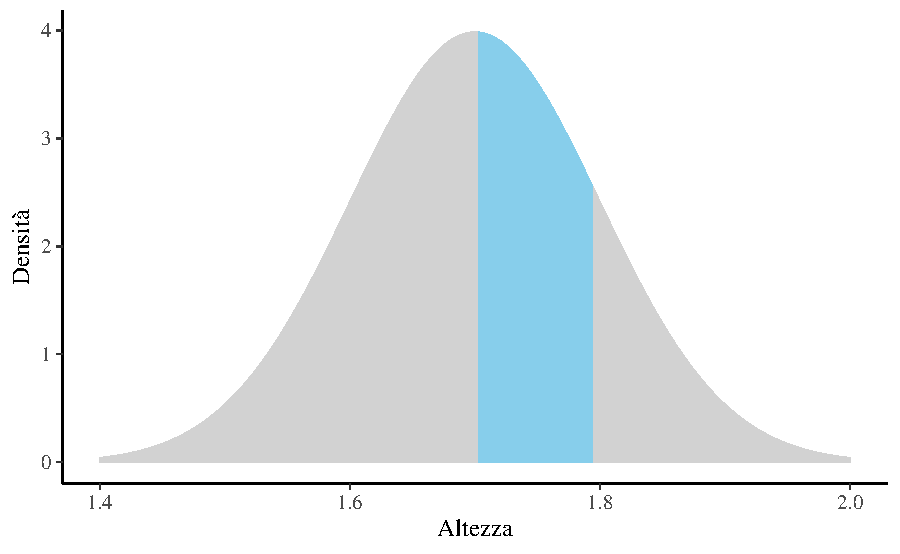
\includegraphics[width=0.8\linewidth]{092_loo_files/figure-latex/unnamed-chunk-6-1} \end{center}

\noindent
La figura mostra che questa relazione non è lineare, è infatti leggermente sublineare. Questo ha senso dato che abbiamo usato una funzione logaritmica.
\end{example}

\hypertarget{entropia-di-una-variabile-casuale}{%
\subsection{Entropia di una variabile casuale}\label{entropia-di-una-variabile-casuale}}

È possibile quantificare la quantità di informazione fornita da una variabile casuale.

\begin{definition}
Sia \(Y = y_1, \dots, y_n\) una variabile casuale e \(p_t(y)\) una distribuzione di probabilità su \(Y\). Si definisce la sua entropia (detta di Shannon) come:
\begin{equation}
H(Y) = - \sum_{i=1}^n p_t(y_i) \cdot \log_2 p_t(y_i).
\label{eq:entropy}
\end{equation}
\end{definition}

\hypertarget{proprietuxe0}{%
\subsection{Proprietà}\label{proprietuxe0}}

Si possono evidenziare due proprietà dell'entropia.

\begin{itemize}
\tightlist
\item
  L'entropia aumenta all'aumentare della varianza di una variabile casuale.
\item
  L'entropia aumenta all'aumentare del numero delle possibilità con cui un evento può verificarsi.
\end{itemize}

\begin{example}
Consideriamo un esempio riguardante le previsioni del tempo. Supponiamo che le probabilità di pioggia e sole siano, rispettivamente, \(p_1 = 0.3\) e \(p_2 = 0.7\). Quindi
\[
H(p) = − [p(y_1) \log_2 p(y_1) + p(y_2) \log_2 p(y_2)] \approx 0.61.
\]
\noindent
Svolgendo i calcoli in \(\R\) abbiamo:

\begin{Shaded}
\begin{Highlighting}[]
\NormalTok{p }\OtherTok{\textless{}{-}} \FunctionTok{c}\NormalTok{(}\FloatTok{0.3}\NormalTok{ , }\FloatTok{0.7}\NormalTok{)}
\SpecialCharTok{{-}}\FunctionTok{sum}\NormalTok{(p}\SpecialCharTok{*}\FunctionTok{log}\NormalTok{(p))}
\CommentTok{\#\textgreater{} [1] 0.611}
\end{Highlighting}
\end{Shaded}

\noindent
Se però viviamo a Las Vegas, allora le probabilità di pioggia e sole saranno qualcosa come \(p(y_1) = 0.01\) e \(p(y_2) = 0.99\). In questo secondo caso, l'entropia è 0.06, ovvero, molto minore di prima. Infatti, a Las Vegas non piove quasi mai, per cui quando abbiamo imparato che, in un certo giorno, non ha piovuto, abbiamo imparato molto poco rispetto a quello che già sapevamo in precedenza.
\end{example}

\begin{example}

Abbiamo visto in precedenza che, se gli esiti possibili sono pioggia o sole con \(p(y_1) = 0.7\), \(p(y_2) = 0.3\), allora l'entropia è

\begin{Shaded}
\begin{Highlighting}[]
\SpecialCharTok{{-}}\NormalTok{(}\FloatTok{0.7} \SpecialCharTok{*} \FunctionTok{log}\NormalTok{(}\FloatTok{0.7}\NormalTok{) }\SpecialCharTok{+} \FloatTok{0.3} \SpecialCharTok{*} \FunctionTok{log}\NormalTok{(}\FloatTok{0.3}\NormalTok{))}
\CommentTok{\#\textgreater{} [1] 0.611}
\end{Highlighting}
\end{Shaded}

\noindent
Se gli esiti possibili sono pioggia, neve o sole con \(p(y_1) = 0.7\), \(p(y_2) = 0.15\) e \(p(y_3) = 0.15\), rispettivamente, allora l'entropia sarà maggiore, ovvero pari a 0.82.

\begin{Shaded}
\begin{Highlighting}[]
\SpecialCharTok{{-}}\NormalTok{(}\FloatTok{0.7} \SpecialCharTok{*} \FunctionTok{log}\NormalTok{(}\FloatTok{0.7}\NormalTok{) }\SpecialCharTok{+} \FloatTok{0.15} \SpecialCharTok{*} \FunctionTok{log}\NormalTok{(}\FloatTok{0.15}\NormalTok{) }\SpecialCharTok{+} \FloatTok{0.15} \SpecialCharTok{*} \FunctionTok{log}\NormalTok{(}\FloatTok{0.15}\NormalTok{))}
\CommentTok{\#\textgreater{} [1] 0.819}
\end{Highlighting}
\end{Shaded}

\end{example}

\hypertarget{dallentropia-allaccuratezza}{%
\section{Dall'entropia all'accuratezza}\label{dallentropia-allaccuratezza}}

Il valore assoluto dell'entropia è difficile da interpretare. Vedremo però come sia possibile usare l'entropia per misurare l'accuratezza di un modello statistico. Nello specifico, ci porremo il problema di misurare la distanza tra la distribuzione di probabilità ipotizzata da un modello, chiamiamola \(p_{\mathcal{M}}\), e la distribuzione di probabilità del vero modello generatore dei dati, \(p_t\). La teoria delle probabilità quantifica l'informazione che viene perduta quando \(p_{\mathcal{M}}\) approssima \(p_t\) mediante la \emph{divergenza di Kullback-Liebler}. La divergenza di Kullback-Liebler, denotata con \(D_{KL}(p_t \mid\mid p_{\mathcal{M}})\), misura dunque l'incremento della nostra incertezza quando una distribuzione ``approssimata'' viene usata al posto della ``vera'' distribuzione di probabilità.

\begin{definition}
Per due distribuzioni discrete \(p_t\) e \(p_{\mathcal{M}}\), la divergenza KL di \(p_{\mathcal{M}}\) da \(p_t\) è definita come:
\begin{equation}
D_{KL}(p_t \mid\mid p_{\mathcal{M}}) = \sum_{i=1}^n p_t(y_i) \cdot \left[\log p_t(y_i) - \log p_{\mathcal{M}}(y_i)\right].
\label{eq:kldivergence}
\end{equation}
\end{definition}

La divergenza di Kullback-Liebler introduce un piccolo cambiamento alla \eqref{eq:entropy}: anziché considerare una sola distribuzione di probabilità, \(p_t\), considera anche una approssimazione a tale distribuzione, ovvero \(p_{\mathcal{M}}\). Calcolando la differenza dei logaritmi dei valori delle due distribuzioni si giunge alla \eqref{eq:kldivergence}.

La divergenza KL misura dunque la quantità di informazione che viene perduta quando una distribuzione approssimata viene usata per descrivere le proprietà della distribuzione di riferimento.
Se c'è una perfetta corrispondenza tra le due distribuzioni, \(p_t = p_{\mathcal{M}}\), allora
\[
D_{KL}(p_t \mid\mid p_{\mathcal{M}}) = D_{KL}(p_t \mid\mid p_t) = \sum_{i=1}^n p_t(y_i) \cdot \left[\log p_t(y_i) - \log p_t(y_i)\right] = 0,
\]
ovvvero: nessuna incertezza aggiuntiva viene introdotta se una distribuzione viene usata per rappresentare se stessa. Altrimenti, cioè se \(p_t \neq p_{\mathcal{M}}\), la divergenza KL assume valori nell'intervallo \([0, \infty]\): all'aumentare della differenza tra \(p_{\mathcal{M}}\) e \(p_t\) aumenta il valore \(D_{KL}(p_t \mid\mid p_{\mathcal{M}})\).

\begin{example}
\autocite[da][]{McElreath_rethinking} Sia la distribuzione target \(p = \{0.3, 0.7\}\). Supponiamo che la distribuzione approssimata \(q\) possa assumere valori da \(q = \{0.01, 0.99\}\) a \(q = \{0.99, 0.01\}\). Calcoliamo la divergenza KL.

Le istruzioni \(\R\) sono le seguenti:

\begin{Shaded}
\begin{Highlighting}[]
\NormalTok{t }\OtherTok{\textless{}{-}}
  \FunctionTok{tibble}\NormalTok{(}
    \AttributeTok{p\_1 =}\NormalTok{ .}\DecValTok{3}\NormalTok{,}
    \AttributeTok{p\_2 =}\NormalTok{ .}\DecValTok{7}\NormalTok{,}
    \AttributeTok{q\_1 =} \FunctionTok{seq}\NormalTok{(}\AttributeTok{from =}\NormalTok{ .}\DecValTok{01}\NormalTok{, }\AttributeTok{to =}\NormalTok{ .}\DecValTok{99}\NormalTok{, }\AttributeTok{by =}\NormalTok{ .}\DecValTok{01}\NormalTok{)}
\NormalTok{  ) }\SpecialCharTok{\%\textgreater{}\%}
  \FunctionTok{mutate}\NormalTok{(}
    \AttributeTok{q\_2 =} \DecValTok{1} \SpecialCharTok{{-}}\NormalTok{ q\_1}
\NormalTok{  ) }\SpecialCharTok{\%\textgreater{}\%}
  \FunctionTok{mutate}\NormalTok{(}
    \AttributeTok{d\_kl =}\NormalTok{ (p\_1 }\SpecialCharTok{*} \FunctionTok{log}\NormalTok{(p\_1 }\SpecialCharTok{/}\NormalTok{ q\_1)) }\SpecialCharTok{+}\NormalTok{ (p\_2 }\SpecialCharTok{*} \FunctionTok{log}\NormalTok{(p\_2 }\SpecialCharTok{/}\NormalTok{ q\_2))}
\NormalTok{  )}

\FunctionTok{head}\NormalTok{(t)}
\CommentTok{\#\textgreater{} \# A tibble: 6 x 5}
\CommentTok{\#\textgreater{}     p\_1   p\_2   q\_1   q\_2  d\_kl}
\CommentTok{\#\textgreater{}   \textless{}dbl\textgreater{} \textless{}dbl\textgreater{} \textless{}dbl\textgreater{} \textless{}dbl\textgreater{} \textless{}dbl\textgreater{}}
\CommentTok{\#\textgreater{} 1   0.3   0.7  0.01  0.99 0.778}
\CommentTok{\#\textgreater{} 2   0.3   0.7  0.02  0.98 0.577}
\CommentTok{\#\textgreater{} 3   0.3   0.7  0.03  0.97 0.462}
\CommentTok{\#\textgreater{} 4   0.3   0.7  0.04  0.96 0.383}
\CommentTok{\#\textgreater{} 5   0.3   0.7  0.05  0.95 0.324}
\CommentTok{\#\textgreater{} 6   0.3   0.7  0.06  0.94 0.276}
\end{Highlighting}
\end{Shaded}

\noindent
Nella figura seguente sull'asse delle ascisse sono rappresentati i valori \(q\) e sull'asse delle ordinante sono riportati i corrispondenti valori \(D_{KL}\).

\begin{Shaded}
\begin{Highlighting}[]
\NormalTok{t }\SpecialCharTok{\%\textgreater{}\%}
  \FunctionTok{ggplot}\NormalTok{(}\FunctionTok{aes}\NormalTok{(}\AttributeTok{x =}\NormalTok{ q\_1, }\AttributeTok{y =}\NormalTok{ d\_kl)) }\SpecialCharTok{+}
  \FunctionTok{geom\_vline}\NormalTok{(}\AttributeTok{xintercept =}\NormalTok{ .}\DecValTok{3}\NormalTok{, }\AttributeTok{linetype =} \DecValTok{2}\NormalTok{) }\SpecialCharTok{+}
  \FunctionTok{geom\_line}\NormalTok{(}\AttributeTok{size =} \DecValTok{1}\NormalTok{) }\SpecialCharTok{+}
  \FunctionTok{annotate}\NormalTok{(}\AttributeTok{geom =} \StringTok{"text"}\NormalTok{, }\AttributeTok{x =}\NormalTok{ .}\DecValTok{4}\NormalTok{, }\AttributeTok{y =} \FloatTok{1.5}\NormalTok{, }\AttributeTok{label =} \StringTok{"q = p"}\NormalTok{,}
           \AttributeTok{size =} \FloatTok{3.5}\NormalTok{) }\SpecialCharTok{+}
  \FunctionTok{labs}\NormalTok{(}\AttributeTok{x =} \StringTok{"q[1]"}\NormalTok{,}
       \AttributeTok{y =} \StringTok{"Divergenza di q da p"}\NormalTok{)}
\end{Highlighting}
\end{Shaded}

\begin{center}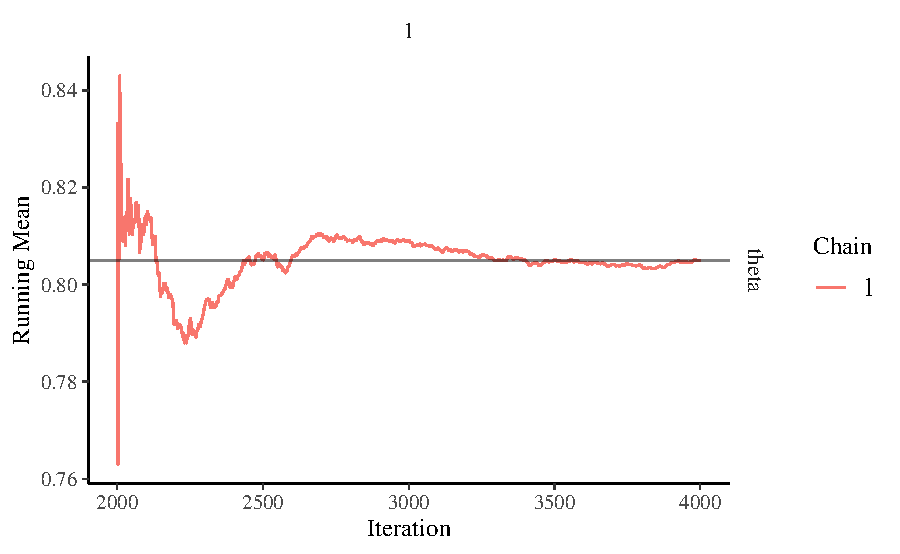
\includegraphics[width=0.8\linewidth]{092_loo_files/figure-latex/unnamed-chunk-11-1} \end{center}

\noindent
Tanto meglio la distribuzione \(q\) approssima la distribuzione target tanto più piccolo è il valore di divergenza KL.
\end{example}

\begin{example}
Sia \(p\) una distribuzione binomiale di parametri \(\theta = 0.2\) e \(n = 5\)

\begin{Shaded}
\begin{Highlighting}[]
\NormalTok{n }\OtherTok{\textless{}{-}} \DecValTok{4}
\NormalTok{p }\OtherTok{\textless{}{-}} \FloatTok{0.2}
\NormalTok{true\_py }\OtherTok{\textless{}{-}} \FunctionTok{dbinom}\NormalTok{(}\DecValTok{0}\SpecialCharTok{:}\NormalTok{n, n, }\FloatTok{0.2}\NormalTok{)}
\NormalTok{true\_py}
\CommentTok{\#\textgreater{} [1] 0.4096 0.4096 0.1536 0.0256 0.0016}
\end{Highlighting}
\end{Shaded}

\noindent
Sia \(q_1\) una approssimazione a \(p\):

\begin{Shaded}
\begin{Highlighting}[]
\NormalTok{q1 }\OtherTok{\textless{}{-}} \FunctionTok{c}\NormalTok{(}\FloatTok{0.46}\NormalTok{, }\FloatTok{0.42}\NormalTok{, }\FloatTok{0.10}\NormalTok{, }\FloatTok{0.01}\NormalTok{, }\FloatTok{0.01}\NormalTok{)}
\NormalTok{q1}
\CommentTok{\#\textgreater{} [1] 0.46 0.42 0.10 0.01 0.01}
\end{Highlighting}
\end{Shaded}

\noindent
Sia \(q_2\) una distribuzione uniforme:

\begin{Shaded}
\begin{Highlighting}[]
\NormalTok{q2 }\OtherTok{\textless{}{-}} \FunctionTok{rep}\NormalTok{(}\FloatTok{0.2}\NormalTok{, }\DecValTok{5}\NormalTok{)}
\NormalTok{q2}
\CommentTok{\#\textgreater{} [1] 0.2 0.2 0.2 0.2 0.2}
\end{Highlighting}
\end{Shaded}

\noindent
La divergenza KL di \(q_1\) da \(p\) è

\begin{Shaded}
\begin{Highlighting}[]
\FunctionTok{sum}\NormalTok{(true\_py }\SpecialCharTok{*} \FunctionTok{log}\NormalTok{(true\_py }\SpecialCharTok{/}\NormalTok{ q1))}
\CommentTok{\#\textgreater{} [1] 0.0293}
\end{Highlighting}
\end{Shaded}

\noindent
La divergenza KL di \(q_2\) da \(p\) è:

\begin{Shaded}
\begin{Highlighting}[]
\FunctionTok{sum}\NormalTok{(true\_py }\SpecialCharTok{*} \FunctionTok{log}\NormalTok{(true\_py }\SpecialCharTok{/}\NormalTok{ q2))}
\CommentTok{\#\textgreater{} [1] 0.486}
\end{Highlighting}
\end{Shaded}

\noindent
È chiaro che perdiamo una quantità maggiore di informazioni se, per descrivere la distribuzione binomiale \(p\), usiamo la distribuzione uniforme \(q_2\) anziché \(q_1\).
\end{example}

\hypertarget{la-divergenza-dipende-dalla-direzione}{%
\subsection{La divergenza dipende dalla direzione}\label{la-divergenza-dipende-dalla-direzione}}

La divergenza KL non è simmetrica: la KL da \(p_t\) a \(p_{\mathcal{M}}\) in generale è diversa dalla KL da \(p_{\mathcal{M}}\) a \(p_t\).

\begin{example}

Usando le seguenti istruzioni \(\R\) otteniamo:

\begin{Shaded}
\begin{Highlighting}[]
\FunctionTok{tibble}\NormalTok{(}\AttributeTok{direction =} \FunctionTok{c}\NormalTok{(}\StringTok{"Da q a p"}\NormalTok{, }\StringTok{"Da p a q"}\NormalTok{),}
       \AttributeTok{p\_1 =} \FunctionTok{c}\NormalTok{(.}\DecValTok{01}\NormalTok{, .}\DecValTok{7}\NormalTok{),}
       \AttributeTok{q\_1 =} \FunctionTok{c}\NormalTok{(.}\DecValTok{7}\NormalTok{, .}\DecValTok{01}\NormalTok{)) }\SpecialCharTok{\%\textgreater{}\%}
  \FunctionTok{mutate}\NormalTok{(}\AttributeTok{p\_2 =} \DecValTok{1} \SpecialCharTok{{-}}\NormalTok{ p\_1,}
         \AttributeTok{q\_2 =} \DecValTok{1} \SpecialCharTok{{-}}\NormalTok{ q\_1) }\SpecialCharTok{\%\textgreater{}\%}
  \FunctionTok{mutate}\NormalTok{(}\AttributeTok{d\_kl =}\NormalTok{ (p\_1 }\SpecialCharTok{*} \FunctionTok{log}\NormalTok{(p\_1 }\SpecialCharTok{/}\NormalTok{ q\_1)) }\SpecialCharTok{+}\NormalTok{ (p\_2 }\SpecialCharTok{*} \FunctionTok{log}\NormalTok{(p\_2 }\SpecialCharTok{/}\NormalTok{ q\_2)))}
\CommentTok{\#\textgreater{} \# A tibble: 2 x 6}
\CommentTok{\#\textgreater{}   direction   p\_1   q\_1   p\_2   q\_2  d\_kl}
\CommentTok{\#\textgreater{}   \textless{}chr\textgreater{}     \textless{}dbl\textgreater{} \textless{}dbl\textgreater{} \textless{}dbl\textgreater{} \textless{}dbl\textgreater{} \textless{}dbl\textgreater{}}
\CommentTok{\#\textgreater{} 1 Da q a p   0.01  0.7   0.99  0.3   1.14}
\CommentTok{\#\textgreater{} 2 Da p a q   0.7   0.01  0.3   0.99  2.62}
\end{Highlighting}
\end{Shaded}

\end{example}

\hypertarget{expected-log-predictive-density}{%
\section{Expected log predictive density}\label{expected-log-predictive-density}}

Nel caso continuo, la divergenza KL diventa:
\begin{equation}
D_{KL}(p_t \mid\mid p_{\mathcal{M}}) = \int_{-\infty}^{+\infty} p_{t}(y) \,\log p_{t}(y) \,\operatorname {d}\!y - \int_{-\infty}^{+\infty}p_{t}(y)\log p_{\mathcal{M}}(y) \,\operatorname {d}\!y.
\label{eq:kl-div-cont}
\end{equation}
Se vengono confrontati due modelli, il primo termine della \eqref{eq:kl-div-cont} resta costante e il confronto si riduce al secondo termine della \eqref{eq:kl-div-cont}, ovvero
\begin{equation}
\int_{-\infty}^{+\infty}p_{t}(y)\log p_{\mathcal{M}}(y) \,\operatorname {d}\!y.
\label{eq:kl-div-cont-t2}
\end{equation}
\noindent
Riscriviamo ora la \eqref{eq:kl-div-cont-t2} facendo riferimento alla distribuzione predittiva a posteriori, \(p(\tilde{y} \mid y)\), perché ciò a cui siamo interessati è la divergenza di \(p(\tilde{y} \mid y)\) da \(p_{t}(y)\):
\begin{equation}
\elpd = \int_{\tilde{y}} p_{t}(\tilde{y}) \log p(\tilde{y} \mid y) \,\operatorname {d}\!\tilde{y}.
\label{eq:elpd}
\end{equation}
La \eqref{eq:elpd} è chiamata \emph{expected log predictive density} (\(\elpd\)) e fornisce la risposta al problema che ci eravamo posti all'inizio di questo Capitolo, ovvero al problema di definire un criterio per valutare la capacità predittiva di un modello. Possiamo pensare alla \eqref{eq:elpd} dicendo che descrive la distribuzione predittiva a posteriori del modello ponderando la verosimiglianza dei possibili dati futuri con la vera distribuzione \(p_t\). Di conseguenza, valori \(\elpd\) più grandi corrispondono ad una maggiore capacità predittiva del modello.

Non dobbiamo preoccuparci di trovare una formulazione analitica della distribuzione predittiva a posteriori \(p(\tilde{y} \mid y)\) perché, come abbiamo visto nel Capitolo \ref{chapter-ppc}, è possibile approssimare tale distribuzione mediante simulazione. Notiamo però che la \eqref{eq:elpd} è formulata nei termini del vero modello generatore dei dati, \(p_t\), il quale, ovviamente, è ignoto.\footnote{Se il modello sottostante i dati fosse noto non avremmo bisogno di cercare il modello migliore, perché \(p_t\) è il modello migliore.} Di conseguenza, la quantità \(\elpd\) non può mai essere calcolata in maniera esatta, ma può essere solo stimata. Il secondo problema di questo Capitolo è capire come la \eqref{eq:elpd} possa essere stimata utilizzando un campione di osservazioni.

\hypertarget{log-pointwise-predictive-density}{%
\subsection{Log pointwise predictive density}\label{log-pointwise-predictive-density}}

Ingenuamente, potremmo pensare di stimare la \eqref{eq:elpd} ipotizzando che la distribuzione del campione coincida con \(p_t\). Usare la distribuzione del campione come proxy del vero modello generatore dei dati (ovvero, ipotizzare che la distribuzione del campione rappresenti fedelmente \(p_t\)) comporta due conseguenze:

\begin{itemize}
\tightlist
\item
  dato che il campione è finito, anziché eseguire un'operazione di integrazione, possiamo semplicemente sommare la densità predittiva a posteriori delle osservazioni;
\item
  non è necessario ponderare per \(p_t\), in quanto assumiamo che la distribuzione empirica del campione corrisponde a \(p_t\) (ciò significa assumere che i valori più comunemente osservati nel campione siano anche quelli più verosimili nella vera distribuzione \(p_t\)).
\end{itemize}

Questo conduce alla seguente equazione:\footnote{In riferimento alla notazione, ricordiamo che \textcite{gelman2014understanding} distinguono tra \(y^{rep}\) e \(\tilde{y}\). I valori \(y^{rep}\) corrispondono ad un'altra possibile realizzazione del medesimo modello statistico che ha prodotto \(y\) mediante determinati valori dei parametri \(\theta\) (repliche sotto lo stesso modello statistico). I valori \(\tilde{y}\) corrispondono invece ad un campione empirico di dati osservato in qualche futura occasione.}
\begin{equation}
\frac{1}{n} \sum_{i=1}^n \log p(y_i^{rep} \mid y).
\label{eq:1n-lppd}
\end{equation}
La quantità \eqref{eq:1n-lppd}, senza il passaggio finale della divisione per il numero di osservazioni, è chiamata \emph{log pointwise predictive density} (\(\lppd\))
\begin{equation}
\lppd = \sum_{i=1}^n \log p(y_i^{rep} \mid y)
\label{eq:lppd}
\end{equation}
e corrisponde alla somma delle densità predittive logaritmiche delle \(n\) osservazioni. Valori più grandi della \eqref{eq:lppd} sono da preferire perché indicano una maggiore accuratezza media. È anche comune vedere espressa la quantità precedente nei termini della \emph{devianza}, ovvero alla \(\lppd\) moltiplicata per -2. In questo secondo caso sono da preferire valori piccoli.

È importante notare che \(\lppd\) fornisce una \emph{sovrastima} della \eqref{eq:elpd}. Tale sovrastima è dovuta al fatto che, nel calcolo della \eqref{eq:lppd}, abbiamo usato \(p(y^{rep} \mid y)\) al posto di \(p(\tilde{y} \mid y)\): in altri termini, abbiamo considerato le osservazioni del campione come se fossero un nuovo campione di dati. In una serie di simulazioni, \textcite{McElreath_rethinking} esamina il significato di questa sovrastima. Nelle simulazioni la devianza viene calcolata come funzione della complessità (ovvero, il numero di parametri) del modello. La simulazione mostra che \(\lppd\) aumenta al crescere del numero di parametri del modello. Ciò significa che \(\lppd\) mostra lo stesso limite del coefficiente di determinazione: aumenta all'aumentare della complessità del modello.

\begin{example}
Esaminiamo un esempio tratto da \href{https://vasishth.github.io/bayescogsci/book/expected-log-predictive-density-of-a-model.html}{Bayesian Data Analysis for Cognitive Science} nel quale la \(\elpd\) viene calcolata in forma esatta oppure mediante approssimazione. Supponiamo di disporre di un campione di \(n\) osservazioni. Supponiamo inoltre di conoscere il vero processo generativo dei dati (qualcosa che in pratica non è mai possibile), ovvero:

\[
p_t(y) = \Beta(1, 3).
\]
I dati sono

\begin{Shaded}
\begin{Highlighting}[]
\FunctionTok{set.seed}\NormalTok{(}\DecValTok{75}\NormalTok{)}
\NormalTok{n }\OtherTok{\textless{}{-}} \DecValTok{10000}
\NormalTok{y\_data }\OtherTok{\textless{}{-}} \FunctionTok{rbeta}\NormalTok{(n, }\DecValTok{1}\NormalTok{, }\DecValTok{3}\NormalTok{)}
\FunctionTok{head}\NormalTok{(y\_data)}
\CommentTok{\#\textgreater{} [1] 0.5506 0.1335 0.8025 0.2143 0.0191 0.0868}
\end{Highlighting}
\end{Shaded}

\noindent
Supponiamo inoltre di avere adattato ai dati un modello bayesiano \(\mathcal{M}\) e di avere ottenuto la distribuzione a posteriori per i parametri del modello. Inoltre, supponiamo di avere derivato la forma analitica della distribuzione predittiva a posteriori per il modello:
\[
p(y^{rep} \mid y) \sim \Beta(2, 2).
\]
Questa distribuzione ci dice quanto sono credibili i possibili dati futuri.

Conoscendo la vera distribuzione dei dati \(p_t(y)\) possiamo calcolare in forma esatta la quantità \(\elpd\), ovvero
\[
\elpd = \int_{y^{rep}}p_{t}(y^{rep})\log p(y^{rep} \mid y) \,\operatorname {d}\!y^{rep}.
\]
\noindent
Svolgiamo i calcoli in \(\R\) otteniamo:

\begin{Shaded}
\begin{Highlighting}[]
\CommentTok{\# True distribution}
\NormalTok{p\_t }\OtherTok{\textless{}{-}} \ControlFlowTok{function}\NormalTok{(y) }\FunctionTok{dbeta}\NormalTok{(y, }\DecValTok{1}\NormalTok{, }\DecValTok{3}\NormalTok{)}
\CommentTok{\# Predictive distribution}
\NormalTok{p }\OtherTok{\textless{}{-}} \ControlFlowTok{function}\NormalTok{(y) }\FunctionTok{dbeta}\NormalTok{(y, }\DecValTok{2}\NormalTok{, }\DecValTok{2}\NormalTok{)}
\CommentTok{\# Integration}
\NormalTok{integrand }\OtherTok{\textless{}{-}} \ControlFlowTok{function}\NormalTok{(y) }\FunctionTok{p\_t}\NormalTok{(y) }\SpecialCharTok{*} \FunctionTok{log}\NormalTok{(}\FunctionTok{p}\NormalTok{(y))}
\FunctionTok{integrate}\NormalTok{(}\AttributeTok{f =}\NormalTok{ integrand, }\AttributeTok{lower =} \DecValTok{0}\NormalTok{, }\AttributeTok{upper =} \DecValTok{1}\NormalTok{)}
\CommentTok{\#\textgreater{} {-}0.375 with absolute error \textless{} 6.8e{-}07}
\end{Highlighting}
\end{Shaded}

\noindent
Tuttavia, in pratica non conosciamo mai \(p_t(y)\). Quindi approssimiamo \(\elpd\) usando la \eqref{eq:elpd}:
\[
\frac{1}{n} \sum_{i=1}^n \log p(y_i \mid y).
\]
\noindent
Così facendo, e svolgendo i calcoli in \(\R\), otteniamo

\begin{Shaded}
\begin{Highlighting}[]
\DecValTok{1}\SpecialCharTok{/}\NormalTok{n }\SpecialCharTok{*} \FunctionTok{sum}\NormalTok{(}\FunctionTok{log}\NormalTok{(}\FunctionTok{p}\NormalTok{(y\_data)))}
\CommentTok{\#\textgreater{} [1] {-}0.364}
\end{Highlighting}
\end{Shaded}

\noindent
un valore diverso da quello trovato in precedenza.
\end{example}

\hypertarget{criterio-di-informazione-e-convalida-incrociata-k-fold}{%
\section{Criterio di informazione e convalida incrociata K-fold}\label{criterio-di-informazione-e-convalida-incrociata-k-fold}}

Nel Paragrafo precedente abbiamo visto che la \eqref{eq:lppd} fornisce una sovrastima della \(\elpd\). Il modo migliore per stimare \(\elpd\) è raccogliere un nuovo campione indipendente di dati, che si ritiene condivida lo stesso processo di generazione dei dati del campione corrente, e stimare \(\elpd\) sul nuovo campione. Questa procedura è chiamata \emph{out-of-sample validation}. Il problema, ovviamente, è che di solito non abbiamo le risorse per raccogliere un nuovo campione. Di conseguenza, gli statistici hanno messo a punto vari metodi per evitare la sovrastima della \(\elpd\) che deriva dal solo utizzo del campione corrente. Ci sono due approcci generali:

\begin{itemize}
\tightlist
\item
  l'introduzione di un fattore di correzione;
\item
  la convalida incrociata cosiddetta K-fold.
\end{itemize}

\hypertarget{aic-dic-e-waic}{%
\subsection{AIC, DIC e WAIC}\label{aic-dic-e-waic}}

Allo scopo di evitare la sovrastima della \eqref{eq:lppd}, le statistiche \emph{Akaike Information Criterion} (AIC), \emph{Deviance Information Criterion} (DIC) e \emph{Widely Applicable Information Criterion} (WAIC) introducono un fattore di correzione. Le statistiche DIC e WAIC sono più complesse di AIC, ma producono un'approssimazione migliore. Tuttavia, i valori AIC, DIC e WAIC sono spesso molto simili tra loro. Per convenienza, dunque, qui ci accontenteremo di esaminare da vicino la statistica più semplice, ovvero AIC.

\hypertarget{criterio-dinformazione-di-akaike}{%
\subsubsection{Criterio d'informazione di Akaike}\label{criterio-dinformazione-di-akaike}}

Il criterio d'informazione di Akaike (in inglese \emph{Akaike information criterion}, indicato come AIC) fornisce un metodo molto semplice per stimare la devianza media \emph{out-of-sample}.

\begin{definition}
Il criterio d'informazione di Akaike è definito come

\begin{equation}
AIC = -2 \log p(y \mid \hat{\theta}_{MLE}) + 2k,
\end{equation}
dove \(k\) è il numero di parametri stimati nel modello e \(p(y \mid \hat{\theta}_{MLE})\) è il valore massimizzato della funzione di verosimiglianza del modello stimato.
\end{definition}

\noindent
Dividendo per -2, otteniamo \(\elpd_{AIC}\):

\begin{equation}
\widehat{\elpd}_{AIC} = \log p(y \mid \hat{\theta}_{MLE}) - k,
\end{equation}

\noindent
dove \(k\) è il fattore di correzione introdotto per evitare la sovrastima discussa in precedenza.

AIC è di interesse principalmente storico e produce una approssimazione attendibile di \(\elpd\) quando:

\begin{enumerate}
\def\labelenumi{\arabic{enumi}.}
\tightlist
\item
  le distribuzioni a priori sono non informative;
\item
  la distribuzione a posteriori è approssimativamente gaussiana multivariata;
\item
  la dimensione \(n\) del campione è molto maggiore del numero \(k\) dei parametri.
\end{enumerate}

\begin{example}

Per meglio comprendere la statistica \(\widehat{\elpd}_{AIC}\), esaminiamo un esempio discusso da \textcite{gelman2014understanding}. Sia \(y_1, \dots, y_n \sim \mathcal{N}(\theta, 1)\) un campione di osservazioni. Nel caso di una distribuzione a priori non-informativa \(p(\theta) \propto 1\), la stima di massima verosimiglianza è \(\bar{y}\). La log-verosimiglianza è
\begin{align}
\log p(y \mid \hat{\theta}_{MLE}) &= -\frac{n}{2} \log (2\pi) - \frac{1}{2}\sum_{i=1}^n (y_i - \bar{y})^2 \notag\\
&= -\frac{n}{2} \log (2\pi) - \frac{1}{2} (n-1)s_y^2,
\end{align}
\noindent
dove \(s_y^2\) è la varianza campionaria.

Nel caso di un modello Normale con con varianza nota e una distribuzione a priori uniforme viene stimato un solo parametro, per cui
\begin{align}
\widehat{\elpd}_{AIC} &= \log p(y \mid \hat{\theta}_{MLE}) - k \notag \\
&= -\frac{n}{2} \log (2\pi) - \frac{1}{2} (n-1)s_y^2 - 1.
\end{align}

\end{example}

\hypertarget{convalida-incrociata-k-fold}{%
\subsection{Convalida incrociata K-fold}\label{convalida-incrociata-k-fold}}

La sovrastima della \eqref{eq:lppd} può anche essere evitata usando una tecnica chiamata \emph{K-fold cross-validation}. Mediante questo metodo vengono stimati i parametri del modello tralasciando una porzione di osservazioni (chiamata \emph{fold}) dal campione per poi valutare il modello sulle osservazioni che sono state escluse. Una stima complessiva dell'accuratezza si ottiene poi calcolando la media del punteggio di accuratezza ottenuto in ogni fold. Il numero minimo di fold è 2; all'altro estremo, è possibile impiegare una singola osservazione in ciascun fold e adattare il modello tante volte (\(n\)) quante sono le singole osservazioni. Questa strategia è chiamata \emph{leave-one-out cross-validation} (LOO-CV).

\hypertarget{importance-sampling}{%
\subsubsection{Importance sampling}\label{importance-sampling}}

La strategia LOO-CV è computazionalmente onerosa (ovvero, richiede un tempo di esecuzione molto lungo). È però possibile approssimare LOO-CV mediante un metodo chiamato \emph{Pareto-smoothed importance sampling cross-validation} {[}PSIS; \textcite{vehtari2017practical}{]}. Tralasciando qui i dettagli matematici, l'intuizione di base è che PSIS fa leva sul punteggio di ``importanza'' posseduto da ciascuna osservazione all'interno della distribuzione a posteriori. Per ``importanza'' si intende il fatto che alcune osservazioni hanno un impatto maggiore sulle proprietà della distribuzione a posteriori di altre: se viene rimossa un'osservazione importante, le proprietà della distribuzione a posteriori cambiano molto; se viene rimossa un'osservazione poco importante, la distribuzione a posteriori cambia poco.
L'``importanza'' così intesa viene chiamata ``peso'' (\emph{weight}) e tali pesi vengono utilizzati per stimare l'accuratezza \emph{out-of-sample} del modello.
PSIS-LOO-CV richiede che il modello venga adattato una volta soltanto ai dati e fornisce una stima della devianza \emph{out-of-sample} che evita la sovrastima della \eqref{eq:lppd}. Inoltre, PSIS-LOO-CV fornisce un feedback sulla propria affidabilità identificando le osservazioni i cui pesi molto elevati potrebbero rendere imprecisa la predizione.

Valori \(\widehat{\elpd}_{\LOO}\) più grandi indicano una maggiore accuratezza predittiva. In alternativa, anziché considerare \(\widehat{\elpd}\), è possibile usare la quantità \(-2 \cdot \widehat{\elpd}\),
la quale è chiamata \emph{LOO Information Criterion} (LOOIC). In questo secondo caso, valori LOOIC più piccoli sono da preferire.

La quantità \(\widehat{\elpd}_{\LOO}\) viene calcolata dai pacchetti \texttt{loo} e \texttt{brms} ed è chiamata \texttt{elpd\_loo} o \texttt{elpd\_kfold}. È anche possibile calcolare la differenza della quantità \texttt{elpd\_loo} per modelli alternativi, insieme alla deviazione standard della distribuzione campionaria di tale differenza.

\hypertarget{confronto-tra-aic-e-loo-cv}{%
\subsubsection{Confronto tra AIC e LOO-CV}\label{confronto-tra-aic-e-loo-cv}}

Per fare un esempio, faremo qui un confronto tra \(\widehat{\elpd}_{AIC}\) e \(\widehat{\elpd}_{LOO-CV}\). Esaminiamo nuovamente l'associazione tra il QI dei figli e il QI delle madri nel campione di dati discusso da \textcite{gelman2020regression}. Una tale relazione può essere descritta da un modello di regressione nel quale la \(y\) corrisponde al QI dei figli e la \(x\) al QI delle madri.

Leggiamo i dati in \R:

\begin{Shaded}
\begin{Highlighting}[]
\FunctionTok{library}\NormalTok{(}\StringTok{"foreign"}\NormalTok{)}
\NormalTok{df }\OtherTok{\textless{}{-}} \FunctionTok{read.dta}\NormalTok{(}\FunctionTok{here}\NormalTok{(}\StringTok{"data"}\NormalTok{, }\StringTok{"kidiq.dta"}\NormalTok{))}
\NormalTok{df}\SpecialCharTok{$}\NormalTok{y }\OtherTok{\textless{}{-}} \FunctionTok{scale}\NormalTok{(df}\SpecialCharTok{$}\NormalTok{kid\_score)[, }\DecValTok{1}\NormalTok{]}
\NormalTok{df}\SpecialCharTok{$}\NormalTok{x1 }\OtherTok{\textless{}{-}} \FunctionTok{scale}\NormalTok{(df}\SpecialCharTok{$}\NormalTok{mom\_iq)[, }\DecValTok{1}\NormalTok{]}
\FunctionTok{head}\NormalTok{(df)}
\CommentTok{\#\textgreater{}   kid\_score mom\_hs mom\_iq mom\_work mom\_age       y      x1}
\CommentTok{\#\textgreater{} 1        65      1  121.1        4      27 {-}1.0679  1.4078}
\CommentTok{\#\textgreater{} 2        98      1   89.4        4      25  0.5489 {-}0.7092}
\CommentTok{\#\textgreater{} 3        85      1  115.4        4      27 {-}0.0881  1.0295}
\CommentTok{\#\textgreater{} 4        83      1   99.4        3      25 {-}0.1860 {-}0.0367}
\CommentTok{\#\textgreater{} 5       115      1   92.7        4      27  1.3818 {-}0.4836}
\CommentTok{\#\textgreater{} 6        98      0  107.9        1      18  0.5489  0.5268}
\end{Highlighting}
\end{Shaded}

Dato che AIC non è una statistica bayesiana, può essere calcolata mediante strumenti frequentisti:

\begin{Shaded}
\begin{Highlighting}[]
\NormalTok{m1\_freq }\OtherTok{\textless{}{-}} \FunctionTok{lm}\NormalTok{(y }\SpecialCharTok{\textasciitilde{}}\NormalTok{ x1, }\AttributeTok{data =}\NormalTok{ df)}
\FunctionTok{AIC}\NormalTok{(m1\_freq) }\SpecialCharTok{/} \SpecialCharTok{{-}}\DecValTok{2}
\CommentTok{\#\textgreater{} [1] {-}570}
\end{Highlighting}
\end{Shaded}

Per ottenere LOO-CV adattiamo ai dati un modello di regressione bayesiano:

\begin{Shaded}
\begin{Highlighting}[]
\NormalTok{modelString }\OtherTok{=} \StringTok{"}
\StringTok{data \{}
\StringTok{  int\textless{}lower=0\textgreater{} N;}
\StringTok{  vector[N] x1;}
\StringTok{  vector[N] y;}
\StringTok{\}}
\StringTok{parameters \{}
\StringTok{  real alpha;}
\StringTok{  real beta1;}
\StringTok{  real\textless{}lower=0\textgreater{} sigma;}
\StringTok{\}}
\StringTok{transformed parameters \{}
\StringTok{  vector[N] mu;}
\StringTok{  for (n in 1:N)\{}
\StringTok{    mu[n] = alpha + beta1*x1[n];}
\StringTok{  \}}
\StringTok{\}}
\StringTok{model \{}
\StringTok{  alpha \textasciitilde{} normal(0, 1);}
\StringTok{  beta1 \textasciitilde{} normal(0, 1);}
\StringTok{  sigma \textasciitilde{} cauchy(0, 1);}
\StringTok{  y \textasciitilde{} normal(mu, sigma);}
\StringTok{\}}
\StringTok{generated quantities \{}
\StringTok{  vector[N] y\_rep;}
\StringTok{  vector[N] log\_lik;}
\StringTok{  for (n in 1:N)\{}
\StringTok{    y\_rep[n] = normal\_rng(mu[n], sigma);}
\StringTok{    log\_lik[n] = normal\_lpdf(y[n] | x1[n] * beta1, sigma);}
\StringTok{  \}}
\StringTok{\}}
\StringTok{"}
\FunctionTok{writeLines}\NormalTok{(modelString, }\AttributeTok{con =} \StringTok{"code/simplereg.stan"}\NormalTok{)}
\end{Highlighting}
\end{Shaded}

\begin{Shaded}
\begin{Highlighting}[]
\NormalTok{data1\_list }\OtherTok{\textless{}{-}} \FunctionTok{list}\NormalTok{(}
  \AttributeTok{N =} \FunctionTok{length}\NormalTok{(df}\SpecialCharTok{$}\NormalTok{kid\_score),}
  \AttributeTok{y =}\NormalTok{ df}\SpecialCharTok{$}\NormalTok{y,}
  \AttributeTok{x1 =}\NormalTok{ df}\SpecialCharTok{$}\NormalTok{x1}
\NormalTok{)}
\end{Highlighting}
\end{Shaded}

\begin{Shaded}
\begin{Highlighting}[]
\NormalTok{file1 }\OtherTok{\textless{}{-}} \FunctionTok{file.path}\NormalTok{(}\StringTok{"code"}\NormalTok{, }\StringTok{"simplereg.stan"}\NormalTok{)}
\end{Highlighting}
\end{Shaded}

\begin{Shaded}
\begin{Highlighting}[]
\NormalTok{mod1 }\OtherTok{\textless{}{-}} \FunctionTok{cmdstan\_model}\NormalTok{(file1)}
\end{Highlighting}
\end{Shaded}

\noindent
Eseguiamo il campionamento MCMC:

\begin{Shaded}
\begin{Highlighting}[]
\NormalTok{fit1 }\OtherTok{\textless{}{-}}\NormalTok{ mod1}\SpecialCharTok{$}\FunctionTok{sample}\NormalTok{(}
  \AttributeTok{data =}\NormalTok{ data1\_list,}
  \AttributeTok{iter\_sampling =}\NormalTok{ 4000L,}
  \AttributeTok{iter\_warmup =}\NormalTok{ 2000L,}
  \AttributeTok{seed =}\NormalTok{ SEED,}
  \AttributeTok{chains =}\NormalTok{ 4L,}
  \AttributeTok{parallel\_chains =}\NormalTok{ 2L,}
  \AttributeTok{refresh =} \DecValTok{0}\NormalTok{,}
  \AttributeTok{thin =} \DecValTok{1}
\NormalTok{)}
\end{Highlighting}
\end{Shaded}

\noindent
Calcoliamo infine la quantità \(\widehat{\elpd}_{LOO-CV}\):

\begin{Shaded}
\begin{Highlighting}[]
\NormalTok{loo1\_result }\OtherTok{\textless{}{-}}\NormalTok{ fit1}\SpecialCharTok{$}\FunctionTok{loo}\NormalTok{(}\AttributeTok{cores =} \DecValTok{4}\NormalTok{)}
\FunctionTok{print}\NormalTok{(loo1\_result)}
\CommentTok{\#\textgreater{} }
\CommentTok{\#\textgreater{} Computed from 16000 by 434 log{-}likelihood matrix}
\CommentTok{\#\textgreater{} }
\CommentTok{\#\textgreater{}          Estimate   SE}
\CommentTok{\#\textgreater{} elpd\_loo   {-}568.6 14.5}
\CommentTok{\#\textgreater{} p\_loo         1.9  0.2}
\CommentTok{\#\textgreater{} looic      1137.2 28.9}
\CommentTok{\#\textgreater{} {-}{-}{-}{-}{-}{-}}
\CommentTok{\#\textgreater{} Monte Carlo SE of elpd\_loo is 0.0.}
\CommentTok{\#\textgreater{} }
\CommentTok{\#\textgreater{} All Pareto k estimates are good (k \textless{} 0.5).}
\CommentTok{\#\textgreater{} See help(\textquotesingle{}pareto{-}k{-}diagnostic\textquotesingle{}) for details.}
\end{Highlighting}
\end{Shaded}

\noindent
Si noti la somiglianza tra \(\widehat{\elpd}_{LOO-CV}\) e \(\widehat{\elpd}_{AIC}\). In conclusione, possiamo dunque dire che \(\widehat{\elpd}_{LOO-CV}\) è la risposta bayesiana allo stesso problema che trova una soluzione frequentista nella statistica \(\widehat{\elpd}_{AIC}\).

\hypertarget{confronto-tra-modelli-mediante-loo-cv}{%
\subsection{Confronto tra modelli mediante LOO-CV}\label{confronto-tra-modelli-mediante-loo-cv}}

Come menzionato in precedenza, l'obiettivo centrale della misurazione dell'accuratezza predittiva è il confronto di modelli. Una volta capito come calcolare LOO-CV con un condice scritto in linguaggio Stan, svolgeremo ora un confronto di modelli.\footnote{A questo proposito, è necessario aggiungere una nota di cautela. Come fa notare \textcite{McElreath_rethinking}, fare previsioni e inferire i rapporti causali sono due cose molto diverse. Statistiche quali AIC, WAIC e LOO-CV consentono di individuare modelli con buone capacità predittive. Tali modelli, tuttavia, non riflettono necessariamente la struttura causale del fenomeno considerato: la selezione di modelli basata unicamente sull'accuratezza predittiva non garantisce che venga selezionato il modello che riflette la struttura causale del fenomeno \autocite[si veda anche][]{navarro2019between}.}

Considereremo qui un confronto di modelli di regressione. Il modello di regressione discusso nel Paragrafo precedente prevede il QI dei bambini dal QI delle madri. Aggiungiamo a tale modello un secondo predittore che corrisponde all'età della madre. L'aggiunta di tale predittore migliori l'accuratezza predittiva del modello?

\begin{Shaded}
\begin{Highlighting}[]
\NormalTok{modelString }\OtherTok{=} \StringTok{"}
\StringTok{data \{}
\StringTok{  int\textless{}lower=0\textgreater{} N;}
\StringTok{  vector[N] x1;}
\StringTok{  vector[N] x2;}
\StringTok{  vector[N] y;}
\StringTok{\}}
\StringTok{parameters \{}
\StringTok{  real alpha;}
\StringTok{  real beta1;}
\StringTok{  real beta2;}
\StringTok{  real\textless{}lower=0\textgreater{} sigma;}
\StringTok{\}}
\StringTok{transformed parameters \{}
\StringTok{  vector[N] mu;}
\StringTok{  for (n in 1:N)\{}
\StringTok{    mu[n] = alpha + beta1*x1[n] + beta2*x2[n];}
\StringTok{  \}}
\StringTok{\}}
\StringTok{model \{}
\StringTok{  alpha \textasciitilde{} normal(0, 1);}
\StringTok{  beta1 \textasciitilde{} normal(0, 1);}
\StringTok{  beta2 \textasciitilde{} normal(0, 1);}
\StringTok{  sigma \textasciitilde{} cauchy(0, 1);}
\StringTok{  y \textasciitilde{} normal(mu, sigma);}
\StringTok{\}}
\StringTok{generated quantities \{}
\StringTok{  vector[N] y\_rep;}
\StringTok{  vector[N] log\_lik;}
\StringTok{  for (n in 1:N)\{}
\StringTok{    y\_rep[n] = normal\_rng(mu[n], sigma);}
\StringTok{    log\_lik[n] = normal\_lpdf(y[n] | x1[n] * beta1 + x2[n] * beta2, sigma);}
\StringTok{  \}}
\StringTok{\}}
\StringTok{"}
\FunctionTok{writeLines}\NormalTok{(modelString, }\AttributeTok{con =} \StringTok{"code/mreg2.stan"}\NormalTok{)}
\end{Highlighting}
\end{Shaded}

\begin{Shaded}
\begin{Highlighting}[]
\NormalTok{df}\SpecialCharTok{$}\NormalTok{x2 }\OtherTok{\textless{}{-}} \FunctionTok{scale}\NormalTok{(df}\SpecialCharTok{$}\NormalTok{mom\_age)[, }\DecValTok{1}\NormalTok{]}
\end{Highlighting}
\end{Shaded}

\begin{Shaded}
\begin{Highlighting}[]
\NormalTok{data2\_list }\OtherTok{\textless{}{-}} \FunctionTok{list}\NormalTok{(}
  \AttributeTok{N =} \FunctionTok{length}\NormalTok{(df}\SpecialCharTok{$}\NormalTok{kid\_score),}
  \AttributeTok{y =}\NormalTok{ df}\SpecialCharTok{$}\NormalTok{y,}
  \AttributeTok{x1 =}\NormalTok{ df}\SpecialCharTok{$}\NormalTok{x1,}
  \AttributeTok{x2 =}\NormalTok{ df}\SpecialCharTok{$}\NormalTok{x2}
\NormalTok{)}
\end{Highlighting}
\end{Shaded}

\begin{Shaded}
\begin{Highlighting}[]
\NormalTok{file2 }\OtherTok{\textless{}{-}} \FunctionTok{file.path}\NormalTok{(}\StringTok{"code"}\NormalTok{, }\StringTok{"mreg2.stan"}\NormalTok{)}
\end{Highlighting}
\end{Shaded}

\begin{Shaded}
\begin{Highlighting}[]
\CommentTok{\# compile model}
\NormalTok{mod2 }\OtherTok{\textless{}{-}} \FunctionTok{cmdstan\_model}\NormalTok{(file2)}
\end{Highlighting}
\end{Shaded}

\begin{Shaded}
\begin{Highlighting}[]
\CommentTok{\# Running MCMC}
\NormalTok{fit2 }\OtherTok{\textless{}{-}}\NormalTok{ mod2}\SpecialCharTok{$}\FunctionTok{sample}\NormalTok{(}
  \AttributeTok{data =}\NormalTok{ data2\_list,}
  \AttributeTok{iter\_sampling =}\NormalTok{ 4000L,}
  \AttributeTok{iter\_warmup =}\NormalTok{ 2000L,}
  \AttributeTok{seed =}\NormalTok{ SEED,}
  \AttributeTok{chains =}\NormalTok{ 4L,}
  \AttributeTok{parallel\_chains =}\NormalTok{ 2L,}
  \AttributeTok{refresh =} \DecValTok{0}\NormalTok{,}
  \AttributeTok{thin =} \DecValTok{1}
\NormalTok{)}
\end{Highlighting}
\end{Shaded}

\begin{Shaded}
\begin{Highlighting}[]
\NormalTok{fit2}\SpecialCharTok{$}\FunctionTok{summary}\NormalTok{(}\FunctionTok{c}\NormalTok{(}\StringTok{"alpha"}\NormalTok{, }\StringTok{"beta1"}\NormalTok{, }\StringTok{"beta2"}\NormalTok{, }\StringTok{"sigma"}\NormalTok{))}
\CommentTok{\#\textgreater{} \# A tibble: 4 x 10}
\CommentTok{\#\textgreater{}   variable     mean  median     sd    mad      q5    q95  rhat ess\_bulk ess\_tail}
\CommentTok{\#\textgreater{}   \textless{}chr\textgreater{}       \textless{}dbl\textgreater{}   \textless{}dbl\textgreater{}  \textless{}dbl\textgreater{}  \textless{}dbl\textgreater{}   \textless{}dbl\textgreater{}  \textless{}dbl\textgreater{} \textless{}dbl\textgreater{}    \textless{}dbl\textgreater{}    \textless{}dbl\textgreater{}}
\CommentTok{\#\textgreater{} 1 alpha    0.000387 5.70e{-}4 0.0431 0.0427 {-}0.0706 0.0709  1.00   18092.   12482.}
\CommentTok{\#\textgreater{} 2 beta1    0.442    4.42e{-}1 0.0434 0.0428  0.372  0.514   1.00   18884.   12262.}
\CommentTok{\#\textgreater{} 3 beta2    0.0510   5.11e{-}2 0.0431 0.0431 {-}0.0192 0.122   1.00   19099.   12929.}
\CommentTok{\#\textgreater{} 4 sigma    0.896    8.96e{-}1 0.0306 0.0303  0.847  0.947   1.00   18776.   13031.}
\end{Highlighting}
\end{Shaded}

\begin{Shaded}
\begin{Highlighting}[]
\NormalTok{loo2\_result }\OtherTok{\textless{}{-}}\NormalTok{ fit2}\SpecialCharTok{$}\FunctionTok{loo}\NormalTok{(}\AttributeTok{cores =} \DecValTok{4}\NormalTok{)}
\FunctionTok{print}\NormalTok{(loo2\_result)}
\CommentTok{\#\textgreater{} }
\CommentTok{\#\textgreater{} Computed from 16000 by 434 log{-}likelihood matrix}
\CommentTok{\#\textgreater{} }
\CommentTok{\#\textgreater{}          Estimate   SE}
\CommentTok{\#\textgreater{} elpd\_loo   {-}569.0 14.5}
\CommentTok{\#\textgreater{} p\_loo         3.0  0.3}
\CommentTok{\#\textgreater{} looic      1137.9 29.0}
\CommentTok{\#\textgreater{} {-}{-}{-}{-}{-}{-}}
\CommentTok{\#\textgreater{} Monte Carlo SE of elpd\_loo is 0.0.}
\CommentTok{\#\textgreater{} }
\CommentTok{\#\textgreater{} All Pareto k estimates are good (k \textless{} 0.5).}
\CommentTok{\#\textgreater{} See help(\textquotesingle{}pareto{-}k{-}diagnostic\textquotesingle{}) for details.}
\end{Highlighting}
\end{Shaded}

Consideriamo infine un terzo modello che utilizza come predittori, oltre al QI della madre, una variabile dicotomica (codificata 0 o 1) che distingue madri che hanno completato le scuole superiori da quelle che non le hanno completate. Nuovamente, la domanda è se l'aggiunta di tale predittore migliori la capacità predittiva del modello.

\begin{Shaded}
\begin{Highlighting}[]
\NormalTok{modelString }\OtherTok{=} \StringTok{"}
\StringTok{data \{}
\StringTok{  int\textless{}lower=0\textgreater{} N;}
\StringTok{  vector[N] x1;}
\StringTok{  vector[N] x3;}
\StringTok{  vector[N] y;}
\StringTok{\}}
\StringTok{parameters \{}
\StringTok{  real alpha;}
\StringTok{  real beta1;}
\StringTok{  real beta3;}
\StringTok{  real\textless{}lower=0\textgreater{} sigma;}
\StringTok{\}}
\StringTok{transformed parameters \{}
\StringTok{  vector[N] mu;}
\StringTok{  for (n in 1:N)\{}
\StringTok{    mu[n] = alpha + beta1*x1[n] + beta3*x3[n];}
\StringTok{  \}}
\StringTok{\}}
\StringTok{model \{}
\StringTok{  alpha \textasciitilde{} normal(0, 1);}
\StringTok{  beta1 \textasciitilde{} normal(0, 1);}
\StringTok{  beta3 \textasciitilde{} normal(0, 1);}
\StringTok{  sigma \textasciitilde{} cauchy(0, 1);}
\StringTok{  y \textasciitilde{} normal(mu, sigma);}
\StringTok{\}}
\StringTok{generated quantities \{}
\StringTok{  vector[N] y\_rep;}
\StringTok{  vector[N] log\_lik;}
\StringTok{  for (n in 1:N)\{}
\StringTok{    y\_rep[n] = normal\_rng(mu[n], sigma);}
\StringTok{    log\_lik[n] = normal\_lpdf(y[n] | x1[n] * beta1 + x3[n] * beta3, sigma);}
\StringTok{  \}}
\StringTok{\}}
\StringTok{"}
\FunctionTok{writeLines}\NormalTok{(modelString, }\AttributeTok{con =} \StringTok{"code/mreg3.stan"}\NormalTok{)}
\end{Highlighting}
\end{Shaded}

\begin{Shaded}
\begin{Highlighting}[]
\NormalTok{df}\SpecialCharTok{$}\NormalTok{x3 }\OtherTok{\textless{}{-}}\NormalTok{ df}\SpecialCharTok{$}\NormalTok{mom\_hs}
\end{Highlighting}
\end{Shaded}

\begin{Shaded}
\begin{Highlighting}[]
\NormalTok{data3\_list }\OtherTok{\textless{}{-}} \FunctionTok{list}\NormalTok{(}
  \AttributeTok{N =} \FunctionTok{length}\NormalTok{(df}\SpecialCharTok{$}\NormalTok{kid\_score),}
  \AttributeTok{y =}\NormalTok{ df}\SpecialCharTok{$}\NormalTok{y,}
  \AttributeTok{x1 =}\NormalTok{ df}\SpecialCharTok{$}\NormalTok{x1,}
  \AttributeTok{x3 =}\NormalTok{ df}\SpecialCharTok{$}\NormalTok{x3}
\NormalTok{)}
\end{Highlighting}
\end{Shaded}

\begin{Shaded}
\begin{Highlighting}[]
\NormalTok{file3 }\OtherTok{\textless{}{-}} \FunctionTok{file.path}\NormalTok{(}\StringTok{"code"}\NormalTok{, }\StringTok{"mreg3.stan"}\NormalTok{)}
\end{Highlighting}
\end{Shaded}

\begin{Shaded}
\begin{Highlighting}[]
\NormalTok{mod3 }\OtherTok{\textless{}{-}} \FunctionTok{cmdstan\_model}\NormalTok{(file3)}
\end{Highlighting}
\end{Shaded}

\begin{Shaded}
\begin{Highlighting}[]
\NormalTok{fit3 }\OtherTok{\textless{}{-}}\NormalTok{ mod3}\SpecialCharTok{$}\FunctionTok{sample}\NormalTok{(}
  \AttributeTok{data =}\NormalTok{ data3\_list,}
  \AttributeTok{iter\_sampling =}\NormalTok{ 4000L,}
  \AttributeTok{iter\_warmup =}\NormalTok{ 2000L,}
  \AttributeTok{seed =}\NormalTok{ SEED,}
  \AttributeTok{chains =}\NormalTok{ 4L,}
  \AttributeTok{parallel\_chains =}\NormalTok{ 2L,}
  \AttributeTok{refresh =} \DecValTok{0}\NormalTok{,}
  \AttributeTok{thin =} \DecValTok{1}
\NormalTok{)}
\end{Highlighting}
\end{Shaded}

\begin{Shaded}
\begin{Highlighting}[]
\NormalTok{fit3}\SpecialCharTok{$}\FunctionTok{summary}\NormalTok{(}\FunctionTok{c}\NormalTok{(}\StringTok{"alpha"}\NormalTok{, }\StringTok{"beta1"}\NormalTok{, }\StringTok{"beta3"}\NormalTok{, }\StringTok{"sigma"}\NormalTok{))}
\CommentTok{\#\textgreater{} \# A tibble: 4 x 10}
\CommentTok{\#\textgreater{}   variable   mean median     sd    mad     q5     q95  rhat ess\_bulk ess\_tail}
\CommentTok{\#\textgreater{}   \textless{}chr\textgreater{}     \textless{}dbl\textgreater{}  \textless{}dbl\textgreater{}  \textless{}dbl\textgreater{}  \textless{}dbl\textgreater{}  \textless{}dbl\textgreater{}   \textless{}dbl\textgreater{} \textless{}dbl\textgreater{}    \textless{}dbl\textgreater{}    \textless{}dbl\textgreater{}}
\CommentTok{\#\textgreater{} 1 alpha    {-}0.225 {-}0.225 0.0951 0.0939 {-}0.380 {-}0.0673  1.00    7808.    8235.}
\CommentTok{\#\textgreater{} 2 beta1     0.414  0.414 0.0445 0.0440  0.340  0.487   1.00   10200.    9870.}
\CommentTok{\#\textgreater{} 3 beta3     0.287  0.288 0.108  0.106   0.108  0.463   1.00    7832.    8542.}
\CommentTok{\#\textgreater{} 4 sigma     0.890  0.889 0.0300 0.0295  0.842  0.941   1.00   11733.   10064.}
\end{Highlighting}
\end{Shaded}

\begin{Shaded}
\begin{Highlighting}[]
\NormalTok{loo3\_result }\OtherTok{\textless{}{-}}\NormalTok{ fit3}\SpecialCharTok{$}\FunctionTok{loo}\NormalTok{(}\AttributeTok{cores =} \DecValTok{4}\NormalTok{)}
\FunctionTok{print}\NormalTok{(loo3\_result)}
\CommentTok{\#\textgreater{} }
\CommentTok{\#\textgreater{} Computed from 16000 by 434 log{-}likelihood matrix}
\CommentTok{\#\textgreater{} }
\CommentTok{\#\textgreater{}          Estimate   SE}
\CommentTok{\#\textgreater{} elpd\_loo   {-}584.2 16.4}
\CommentTok{\#\textgreater{} p\_loo         7.4  0.6}
\CommentTok{\#\textgreater{} looic      1168.4 32.8}
\CommentTok{\#\textgreater{} {-}{-}{-}{-}{-}{-}}
\CommentTok{\#\textgreater{} Monte Carlo SE of elpd\_loo is 0.0.}
\CommentTok{\#\textgreater{} }
\CommentTok{\#\textgreater{} All Pareto k estimates are good (k \textless{} 0.5).}
\CommentTok{\#\textgreater{} See help(\textquotesingle{}pareto{-}k{-}diagnostic\textquotesingle{}) for details.}
\end{Highlighting}
\end{Shaded}

Per eseguire un confronto tra modelli in termini della loro capacità predittiva esaminiamo la differenza di LOO-CV tra coppie di modelli. Le seguenti istruzioni \(\R\) producono la quantità \texttt{elpd\_diff}, ovvero la differenza tra stime della \(\elpd\) fornite da due modelli. Il primo argomento della funzione \texttt{loo\_compare()} specifica il modello che viene usato come confronto. Nella prima riga dell'output, il valore \texttt{elpd\_diff} è 0 (cioè, \(x − x = 0\)). Nelle righe successive sono riportate le differenze rispetto al modello di confronto (in questo caso, il modello 1). La colonna \texttt{se\_diff} riporta l'errore standard di tali differenze.

L'incertezza della stima dell'accuratezza \emph{out-of-sample} si distribuisce in maniera approssimativamente normale con media uguale al valore riportato dal software e deviazione standard uguale a ciò che è indicato nell'output come errore standard. Quando il campione è piccolo, questa approssimazione produce una forte sottostima dell'incertezza, ma fornisce comunque una stima migliore di AIC, DIC e WAIC.

\begin{Shaded}
\begin{Highlighting}[]
\NormalTok{w }\OtherTok{\textless{}{-}} \FunctionTok{loo\_compare}\NormalTok{(loo1\_result, loo2\_result, loo3\_result)}
\FunctionTok{print}\NormalTok{(w)}
\CommentTok{\#\textgreater{}        elpd\_diff se\_diff}
\CommentTok{\#\textgreater{} model1   0.0       0.0  }
\CommentTok{\#\textgreater{} model2  {-}0.4       1.3  }
\CommentTok{\#\textgreater{} model3 {-}15.6       6.0}
\end{Highlighting}
\end{Shaded}

Per interpretare l'output, usiamo il criterio suggerito da \textcite{gelman1995bayesian}: consideriamo ``credibile'' una differenza se \texttt{elpd\_diff} è almeno due volte maggiore di \texttt{se\_diff}. Nel caso presente, dunque, il confronto tra il modello 2 e il modello 1 indica che la quantità \texttt{elpd\_diff} è molto piccola rispetto al suo errore standard.
Questo accade se un predittore è associato in modo trascurabile con la variabile dipendente. I dati presenti, dunque, non offrono alcuna evidenza che aggiungere dell'età della madre come predittore migliori la capacità predittiva del modello. Nel confronto tra modello 3 e modello 1, invece, la quantità \texttt{elpd\_diff} è maggiore di due volte il valore dell'errore standard. Questo suggerisce un incremento della capacità predittiva del modello quiando il livello di istruzione della madre viene incluso tra i predittori.

È anche possibile calcolare l'intervallo di credibilità per \texttt{elpd\_diff}:

\begin{Shaded}
\begin{Highlighting}[]
\FloatTok{15.5} \SpecialCharTok{+} \FunctionTok{c}\NormalTok{(}\SpecialCharTok{{-}}\DecValTok{1}\NormalTok{, }\DecValTok{1}\NormalTok{) }\SpecialCharTok{*} \FunctionTok{qnorm}\NormalTok{(.}\DecValTok{95}\NormalTok{, }\DecValTok{0}\NormalTok{, }\DecValTok{1}\NormalTok{) }\SpecialCharTok{*} \FloatTok{6.0}
\CommentTok{\#\textgreater{} [1]  5.63 25.37}
\end{Highlighting}
\end{Shaded}

\hypertarget{outlier}{%
\subsection{Outlier}\label{outlier}}

Si è soliti pensare che la maggior parte delle osservazioni del campione sia prodotta da un unico meccanismo generatore dei dati, mentre le rimanenti osservazioni sono la realizzazione di un diverso processo stocastico. Le osservazioni che appartengono a questo secondo gruppo si chiamano \emph{outlier}. È dunque necessario identificare gli outlier e limitare la loro influenza sull'inferenza.\footnote{\textcite{McElreath_rethinking} nota che, spesso, i ricercatori eliminano i valori anomali prima di adattare un modello ai dati, basandosi solo sulla distanza dal valore medio della variabile dipendente misurata in termini di unità di deviazione standard. Secondo \textcite{McElreath_rethinking} questo non dovrebbe mai essere fatto: un'osservazione può essere considerata come un valore anomalo o un valore influente solo alla luce delle predizioni di un modello (mai prima di avere adattato il modello ai dati). Se ci sono solo pochi valori anomali una strategia possibile è quella di riportare i risultati delle analisi statistiche svolte su tutto il campione dei dati oppure dopo avere eliminato le osservazioni anomale e influenti.}

Poniamoci ora il problema di identificare gli outlier con la tecnica PSIS-LOO-CV. Quando PSIS-LOO-CV viene calcolato con il pacchetto \texttt{loo}, l'output riporta il parametro di forma della distribuzione di Pareto (valore \texttt{k}). Tale valore può essere utilizzato per identificare gli outlier. Infatti, il valore \texttt{k} valuta, per ciascun punto del campione, l'approssimazione usata da PSIS-LOO-CV. Se \(k < 0.5\), i pesi di importanza vengono stimati in modo accurato; se il valore \(k\) di Pareto di un punto è \(> 0.7\), i pesi di importanza possono essere inaccurati. Le osservazioni con \(k > 0.7\) sono dunque osservazioni outlier.

Per fare un esempio concreto, introduciamo nel campione dell'esempio precedente una singola osservazione outlier.

\begin{Shaded}
\begin{Highlighting}[]
\NormalTok{df1 }\OtherTok{\textless{}{-}}\NormalTok{ df}
\FunctionTok{dim}\NormalTok{(df1)}
\CommentTok{\#\textgreater{} [1] 434   9}
\NormalTok{df1}\SpecialCharTok{$}\NormalTok{x1[}\DecValTok{434}\NormalTok{] }\OtherTok{\textless{}{-}} \DecValTok{10}
\NormalTok{df1}\SpecialCharTok{$}\NormalTok{y[}\DecValTok{434}\NormalTok{] }\OtherTok{\textless{}{-}} \DecValTok{10}
\end{Highlighting}
\end{Shaded}

\noindent
Sistemiamo i dati nel formato appropriato per Stan:

\begin{Shaded}
\begin{Highlighting}[]
\NormalTok{data1a\_list }\OtherTok{\textless{}{-}} \FunctionTok{list}\NormalTok{(}
  \AttributeTok{N =} \FunctionTok{length}\NormalTok{(df1}\SpecialCharTok{$}\NormalTok{kid\_score),}
  \AttributeTok{y =}\NormalTok{ df1}\SpecialCharTok{$}\NormalTok{y,}
  \AttributeTok{x1 =}\NormalTok{ df1}\SpecialCharTok{$}\NormalTok{x1}
\NormalTok{)}
\end{Highlighting}
\end{Shaded}

\noindent
Adattiamo nuovamente il modello 1 ad un campione di dati che contiene un outlier.

\begin{Shaded}
\begin{Highlighting}[]
\NormalTok{fit1a }\OtherTok{\textless{}{-}}\NormalTok{ mod1}\SpecialCharTok{$}\FunctionTok{sample}\NormalTok{(}
  \AttributeTok{data =}\NormalTok{ data1a\_list,}
  \AttributeTok{iter\_sampling =}\NormalTok{ 4000L,}
  \AttributeTok{iter\_warmup =}\NormalTok{ 2000L,}
  \AttributeTok{seed =}\NormalTok{ SEED,}
  \AttributeTok{chains =}\NormalTok{ 4L,}
  \AttributeTok{parallel\_chains =}\NormalTok{ 2L,}
  \AttributeTok{refresh =} \DecValTok{0}\NormalTok{,}
  \AttributeTok{thin =} \DecValTok{1}
\NormalTok{)}
\end{Highlighting}
\end{Shaded}

\begin{Shaded}
\begin{Highlighting}[]
\NormalTok{loo1a\_result }\OtherTok{\textless{}{-}}\NormalTok{ fit1a}\SpecialCharTok{$}\FunctionTok{loo}\NormalTok{(}\AttributeTok{cores =} \DecValTok{4}\NormalTok{)}
\end{Highlighting}
\end{Shaded}

\noindent
Una tabella diagnostica che riassume le stime dei parametri di forma della distribuzione di Pareto si ottiene nel modo seguente:

\begin{Shaded}
\begin{Highlighting}[]
\FunctionTok{print}\NormalTok{(loo1a\_result)}
\CommentTok{\#\textgreater{} }
\CommentTok{\#\textgreater{} Computed from 16000 by 434 log{-}likelihood matrix}
\CommentTok{\#\textgreater{} }
\CommentTok{\#\textgreater{}          Estimate   SE}
\CommentTok{\#\textgreater{} elpd\_loo   {-}586.6 20.1}
\CommentTok{\#\textgreater{} p\_loo         7.1  5.4}
\CommentTok{\#\textgreater{} looic      1173.2 40.3}
\CommentTok{\#\textgreater{} {-}{-}{-}{-}{-}{-}}
\CommentTok{\#\textgreater{} Monte Carlo SE of elpd\_loo is NA.}
\CommentTok{\#\textgreater{} }
\CommentTok{\#\textgreater{} Pareto k diagnostic values:}
\CommentTok{\#\textgreater{}                          Count Pct.    Min. n\_eff}
\CommentTok{\#\textgreater{} ({-}Inf, 0.5]   (good)     433   99.8\%   9998      }
\CommentTok{\#\textgreater{}  (0.5, 0.7]   (ok)         0    0.0\%   \textless{}NA\textgreater{}      }
\CommentTok{\#\textgreater{}    (0.7, 1]   (bad)        0    0.0\%   \textless{}NA\textgreater{}      }
\CommentTok{\#\textgreater{}    (1, Inf)   (very bad)   1    0.2\%   13        }
\CommentTok{\#\textgreater{} See help(\textquotesingle{}pareto{-}k{-}diagnostic\textquotesingle{}) for details.}
\end{Highlighting}
\end{Shaded}

\noindent
Un grafico che riporta le stime dei parametri di forma della distribuzione di Pareto per ciascuna osservazione è dato da:

\begin{Shaded}
\begin{Highlighting}[]
\FunctionTok{plot}\NormalTok{(loo1a\_result)}
\end{Highlighting}
\end{Shaded}

\begin{center}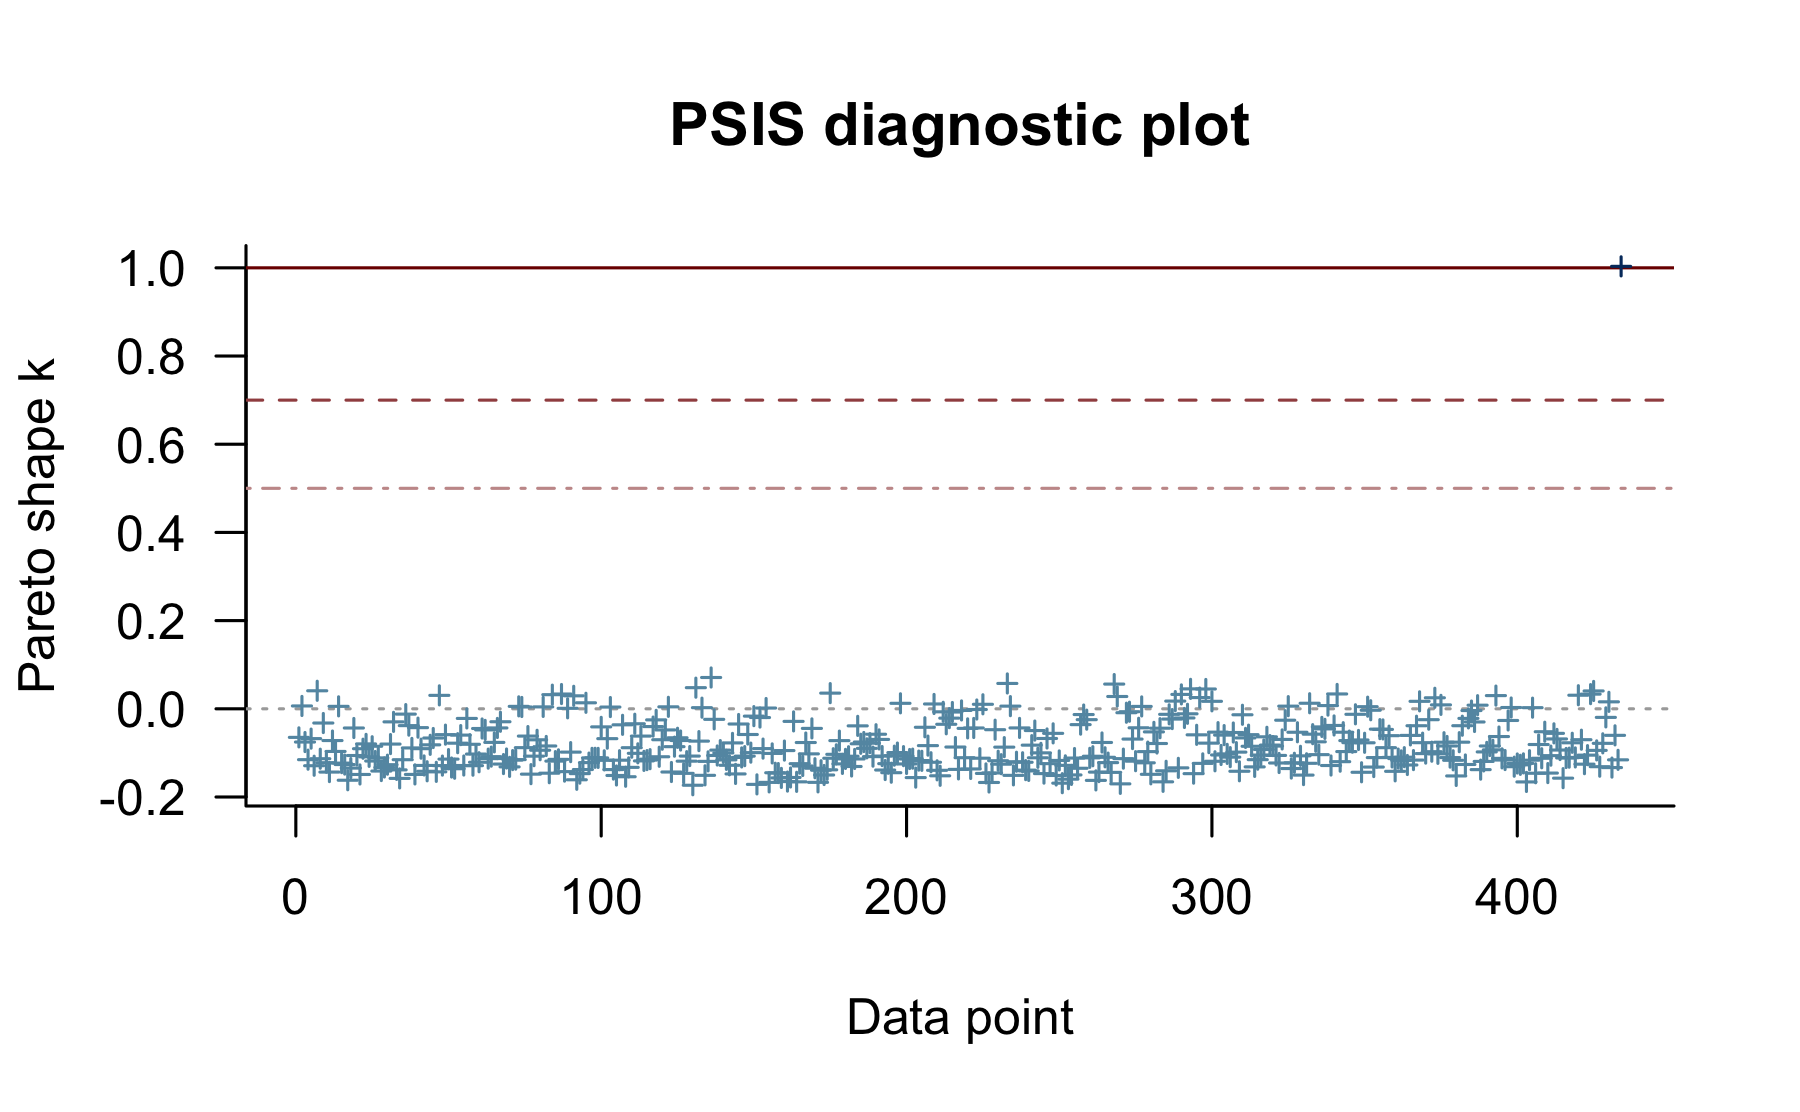
\includegraphics[width=0.8\linewidth]{092_loo_files/figure-latex/unnamed-chunk-52-1} \end{center}

\noindent
Il valore \texttt{k} stimato da PSIS-LOO-CV mette chiaramente in luce il fatto che il valore introdotto nel campione è un outlier. L'indice dell'osservazione outlier è identificato con:

\begin{Shaded}
\begin{Highlighting}[]
\FunctionTok{pareto\_k\_ids}\NormalTok{(loo1a\_result, }\AttributeTok{threshold =} \FloatTok{0.7}\NormalTok{)}
\CommentTok{\#\textgreater{} [1] 434}
\end{Highlighting}
\end{Shaded}

\hypertarget{selezione-di-variabili}{%
\section{Selezione di variabili}\label{selezione-di-variabili}}

I concetti che sono stati introdotti in questo Capitolo, tra le altre cose, risultano utili per affrontare un problema importante in psicologia, ovvero quello della semplificazione di un modello di regressione che contiene molti predittori. Il problema è quello di selezionare un insieme di variabili indipendenti così che tale selezione non comporti una apprezzabile perdita nella capacità predittiva del modello ristretto rispetto al modello completo. Un modo per identificare le variabili rilevanti per prevedere una determinata variabile risposta è quello di utilizzare il metodo basato sulla proiezione, come discusso nel seguente \href{https://cran.r-project.org/web/packages/projpred/vignettes/quickstart.html}{link} e in \textcite{piironen2017comparison}. Per descrivere questa procedura, adatto qui un esempio discusso da Mark Lai in \href{https://bookdown.org/marklhc/notes_bookdown/model-comparison-and-regularization.html}{Course Handouts for Bayesian Data Analysis Class}. Iniziamo a leggere i dati.

\begin{Shaded}
\begin{Highlighting}[]
\NormalTok{kidiq }\OtherTok{\textless{}{-}}\NormalTok{ rio}\SpecialCharTok{::}\FunctionTok{import}\NormalTok{(here}\SpecialCharTok{::}\FunctionTok{here}\NormalTok{(}\StringTok{"data"}\NormalTok{, }\StringTok{"kidiq.dta"}\NormalTok{))}
\NormalTok{kidiq }\OtherTok{\textless{}{-}}\NormalTok{ kidiq }\SpecialCharTok{\%\textgreater{}\%}
  \FunctionTok{mutate}\NormalTok{(}
    \AttributeTok{mom\_hs =} \FunctionTok{factor}\NormalTok{(mom\_hs, }\AttributeTok{labels =} \FunctionTok{c}\NormalTok{(}\StringTok{"no"}\NormalTok{, }\StringTok{"yes"}\NormalTok{))}
\NormalTok{  )}
\end{Highlighting}
\end{Shaded}

\noindent
Per potere usare delle distribuzione a priori sensate per i parametri, standardizzo le variabili numeriche.

\begin{Shaded}
\begin{Highlighting}[]
\NormalTok{scale\_this }\OtherTok{\textless{}{-}} \ControlFlowTok{function}\NormalTok{(x) }\FunctionTok{as.vector}\NormalTok{(}\FunctionTok{scale}\NormalTok{(x))}
\NormalTok{kidiq\_scaled }\OtherTok{\textless{}{-}}\NormalTok{ kidiq }\SpecialCharTok{\%\textgreater{}\%}
  \FunctionTok{as\_tibble}\NormalTok{() }\SpecialCharTok{\%\textgreater{}\%}
  \FunctionTok{mutate}\NormalTok{(}\FunctionTok{across}\NormalTok{(}\FunctionTok{where}\NormalTok{(is.numeric), scale\_this))}
\NormalTok{kidiq\_scaled }\OtherTok{\textless{}{-}}\NormalTok{ kidiq\_scaled }\SpecialCharTok{\%\textgreater{}\%}
  \FunctionTok{mutate}\NormalTok{(}
    \AttributeTok{mom\_hs =}\NormalTok{ kidiq}\SpecialCharTok{$}\NormalTok{mom\_hs}
\NormalTok{  )}
\FunctionTok{glimpse}\NormalTok{(kidiq\_scaled)}
\CommentTok{\#\textgreater{} Rows: 434}
\CommentTok{\#\textgreater{} Columns: 5}
\CommentTok{\#\textgreater{} $ kid\_score \textless{}dbl\textgreater{} {-}1.06793, 0.54887, {-}0.08805, {-}0.18604, 1.38176, 0.54887, {-}0.\textasciitilde{}}
\CommentTok{\#\textgreater{} $ mom\_hs    \textless{}fct\textgreater{} yes, yes, yes, yes, yes, no, yes, yes, yes, yes, yes, yes, y\textasciitilde{}}
\CommentTok{\#\textgreater{} $ mom\_iq    \textless{}dbl\textgreater{} 1.40784, {-}0.70921, 1.02954, {-}0.03669, {-}0.48362, 0.52679, 2.5\textasciitilde{}}
\CommentTok{\#\textgreater{} $ mom\_work  \textless{}dbl\textgreater{} 0.9342, 0.9342, 0.9342, 0.0878, 0.9342, {-}1.6051, 0.9342, 0.0\textasciitilde{}}
\CommentTok{\#\textgreater{} $ mom\_age   \textless{}dbl\textgreater{} 1.5602, 0.8198, 1.5602, 0.8198, 1.5602, {-}1.7718, {-}1.0313, 0.\textasciitilde{}}
\end{Highlighting}
\end{Shaded}

Il seguente modello di regressione utilizza \texttt{kid\_score} quale variabile dipendente e, quali predittori, include tutte le altre variabili disponibili e le loro interazioni a due vie.

\begin{Shaded}
\begin{Highlighting}[]
\NormalTok{m1 }\OtherTok{\textless{}{-}} \FunctionTok{brm}\NormalTok{(}
\NormalTok{  kid\_score }\SpecialCharTok{\textasciitilde{}}\NormalTok{ (mom\_iq }\SpecialCharTok{+}\NormalTok{ mom\_hs }\SpecialCharTok{+}\NormalTok{ mom\_work }\SpecialCharTok{+}\NormalTok{ mom\_age)}\SpecialCharTok{\^{}}\DecValTok{2}\NormalTok{,}
  \AttributeTok{data =}\NormalTok{ kidiq\_scaled,}
  \AttributeTok{prior =} \FunctionTok{c}\NormalTok{(}
    \FunctionTok{prior}\NormalTok{(}\FunctionTok{normal}\NormalTok{(}\DecValTok{0}\NormalTok{, }\DecValTok{1}\NormalTok{), }\AttributeTok{class =} \StringTok{"Intercept"}\NormalTok{),}
    \FunctionTok{prior}\NormalTok{(}\FunctionTok{normal}\NormalTok{(}\DecValTok{0}\NormalTok{, }\DecValTok{1}\NormalTok{), }\AttributeTok{class =} \StringTok{"b"}\NormalTok{),}
    \FunctionTok{prior}\NormalTok{(}\FunctionTok{student\_t}\NormalTok{(}\DecValTok{4}\NormalTok{, }\DecValTok{0}\NormalTok{, }\DecValTok{1}\NormalTok{), }\AttributeTok{class =} \StringTok{"sigma"}\NormalTok{)}
\NormalTok{  ),}
  \AttributeTok{seed =} \DecValTok{2302}\NormalTok{,}
  \AttributeTok{chains =}\NormalTok{ 4L,}
  \AttributeTok{cores =}\NormalTok{ 4L,}
  \AttributeTok{refresh =} \DecValTok{0}\NormalTok{,}
  \AttributeTok{backend =} \StringTok{"cmdstan"}
\NormalTok{)}
\CommentTok{\#\textgreater{} Running MCMC with 4 parallel chains...}
\CommentTok{\#\textgreater{} }
\CommentTok{\#\textgreater{} Chain 1 finished in 0.2 seconds.}
\CommentTok{\#\textgreater{} Chain 2 finished in 0.2 seconds.}
\CommentTok{\#\textgreater{} Chain 3 finished in 0.2 seconds.}
\CommentTok{\#\textgreater{} Chain 4 finished in 0.2 seconds.}
\CommentTok{\#\textgreater{} }
\CommentTok{\#\textgreater{} All 4 chains finished successfully.}
\CommentTok{\#\textgreater{} Mean chain execution time: 0.2 seconds.}
\CommentTok{\#\textgreater{} Total execution time: 0.3 seconds.}
\end{Highlighting}
\end{Shaded}

\noindent
Un grafico che riporta un posterior predictive check si ottiene con l'istruzione seguente:

\begin{Shaded}
\begin{Highlighting}[]
\FunctionTok{pp\_check}\NormalTok{(m1, }\AttributeTok{ndraws =} \DecValTok{50}\NormalTok{, }\AttributeTok{alpha =} \FloatTok{0.5}\NormalTok{) }\SpecialCharTok{+}
  \FunctionTok{xlim}\NormalTok{(}\SpecialCharTok{{-}}\DecValTok{5}\NormalTok{, }\DecValTok{4}\NormalTok{) }\SpecialCharTok{+}
  \FunctionTok{labs}\NormalTok{(}\AttributeTok{x =} \StringTok{"Kid IQ"}\NormalTok{)}
\end{Highlighting}
\end{Shaded}

\begin{center}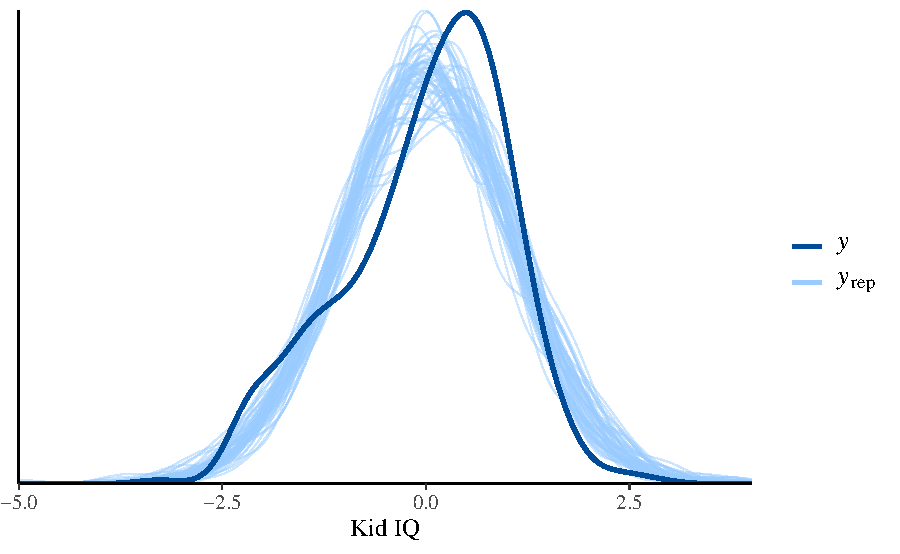
\includegraphics[width=0.8\linewidth]{092_loo_files/figure-latex/unnamed-chunk-57-1} \end{center}

\noindent
Identifichiamo ora l'importanza relativa delle variabili indipendenti nei termini della loro importanza per la previsione:

\begin{Shaded}
\begin{Highlighting}[]
\CommentTok{\# Variable selection}
\NormalTok{vs }\OtherTok{\textless{}{-}}\NormalTok{ projpred}\SpecialCharTok{::}\FunctionTok{varsel}\NormalTok{(m1)}
\end{Highlighting}
\end{Shaded}

\noindent
Un grafico dell'importanza relativa di ciascuna variable per la previsione di \texttt{kid\_score} si ottiene nel modo seguente:

\begin{Shaded}
\begin{Highlighting}[]
\CommentTok{\# plot predictive performance on training data}
\FunctionTok{plot}\NormalTok{(vs, }\AttributeTok{stats =} \FunctionTok{c}\NormalTok{(}\StringTok{"elpd"}\NormalTok{, }\StringTok{"rmse"}\NormalTok{))}
\end{Highlighting}
\end{Shaded}

\begin{center}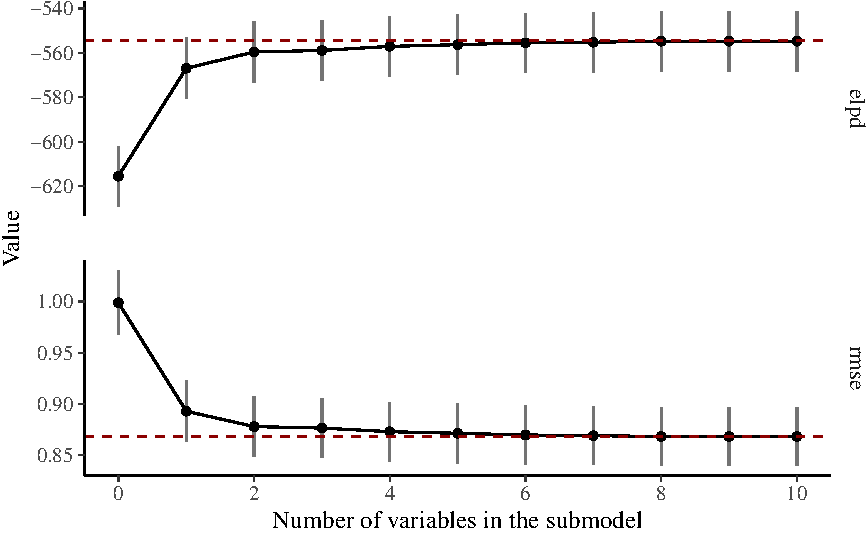
\includegraphics[width=0.8\linewidth]{092_loo_files/figure-latex/unnamed-chunk-58-1} \end{center}

\noindent
Troviamo ora il numero di variabili da mantenere, in base al modello completo:

\begin{Shaded}
\begin{Highlighting}[]
\NormalTok{projpred}\SpecialCharTok{::}\FunctionTok{suggest\_size}\NormalTok{(vs)}
\CommentTok{\#\textgreater{} [1] 5}
\end{Highlighting}
\end{Shaded}

\noindent
Usiamo quindi il metodo \texttt{cv\_varsel()} per eseguire la convalida incrociata per vedere quante variabili dovrebbero essere incluse nel modello:

\begin{Shaded}
\begin{Highlighting}[]
\CommentTok{\# With cross{-}validation}
\NormalTok{cvs }\OtherTok{\textless{}{-}}\NormalTok{ projpred}\SpecialCharTok{::}\FunctionTok{cv\_varsel}\NormalTok{(m1, }\AttributeTok{verbose =} \ConstantTok{FALSE}\NormalTok{)}
\end{Highlighting}
\end{Shaded}

\noindent
In base al metodo della convalida incrociata, il numero di variabili da mantenere è

\begin{Shaded}
\begin{Highlighting}[]
\NormalTok{projpred}\SpecialCharTok{::}\FunctionTok{suggest\_size}\NormalTok{(cvs)}
\CommentTok{\#\textgreater{} [1] 1}
\end{Highlighting}
\end{Shaded}

\noindent
Generiamo il grafico dei risultati della convalida incrociata, questa volta relativi al modello completo:

\begin{Shaded}
\begin{Highlighting}[]
\FunctionTok{plot}\NormalTok{(cvs, }\AttributeTok{stats =} \FunctionTok{c}\NormalTok{(}\StringTok{"elpd"}\NormalTok{, }\StringTok{"rmse"}\NormalTok{), }\AttributeTok{deltas =} \ConstantTok{TRUE}\NormalTok{)}
\end{Highlighting}
\end{Shaded}

\begin{center}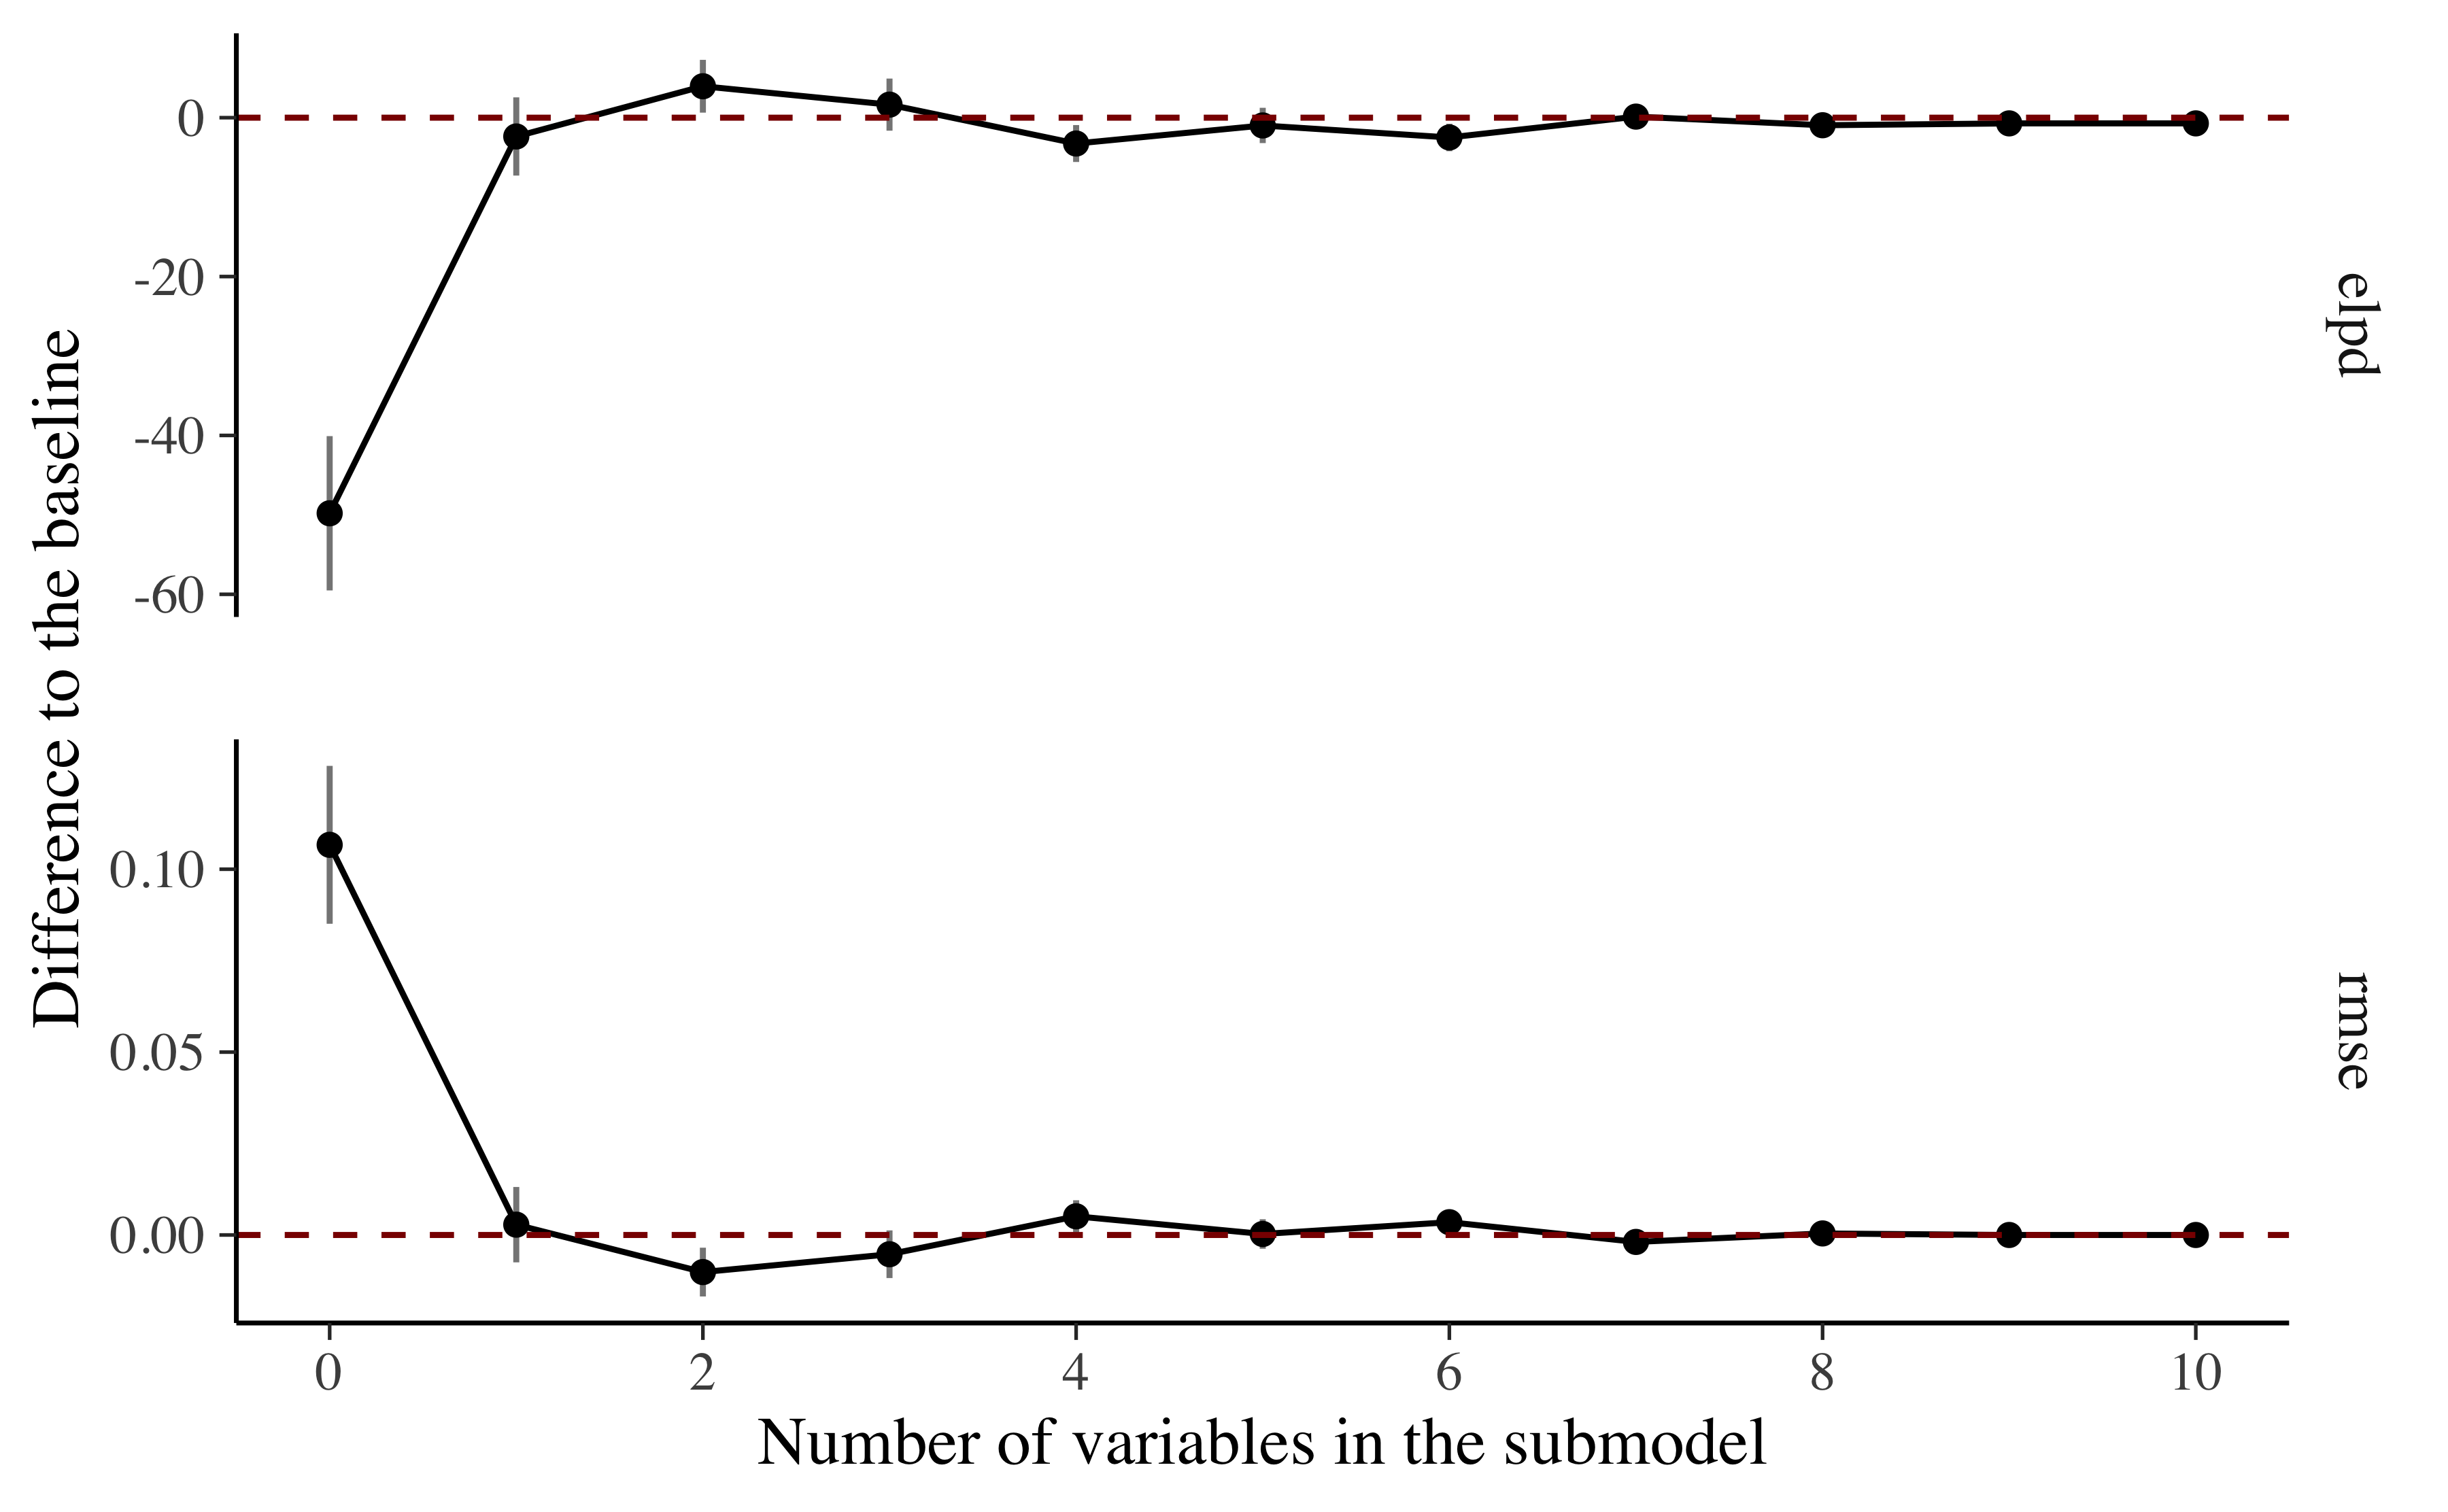
\includegraphics[width=0.8\linewidth]{092_loo_files/figure-latex/unnamed-chunk-61-1} \end{center}

\noindent
Stampiamo l'elenco delle variabili ordinate in base alla loro importanza relativa, secondo il metodo della convalida incrociata:

\begin{Shaded}
\begin{Highlighting}[]
\FunctionTok{summary}\NormalTok{(cvs, }\AttributeTok{stats=}\FunctionTok{c}\NormalTok{(}\StringTok{\textquotesingle{}mse\textquotesingle{}}\NormalTok{), }\AttributeTok{type =} \FunctionTok{c}\NormalTok{(}\StringTok{\textquotesingle{}mean\textquotesingle{}}\NormalTok{,}\StringTok{\textquotesingle{}se\textquotesingle{}}\NormalTok{))}
\CommentTok{\#\textgreater{}    size   solution\_terms   mse mse.se}
\CommentTok{\#\textgreater{} 2     0             \textless{}NA\textgreater{} 1.001 0.0651}
\CommentTok{\#\textgreater{} 3     1           mom\_iq 0.804 0.0536}
\CommentTok{\#\textgreater{} 4     2    mom\_iq:mom\_hs 0.781 0.0519}
\CommentTok{\#\textgreater{} 5     3           mom\_hs 0.790 0.0530}
\CommentTok{\#\textgreater{} 6     4   mom\_hs:mom\_age 0.808 0.0539}
\CommentTok{\#\textgreater{} 7     5  mom\_hs:mom\_work 0.800 0.0541}
\CommentTok{\#\textgreater{} 8     6 mom\_work:mom\_age 0.805 0.0539}
\CommentTok{\#\textgreater{} 9     7  mom\_iq:mom\_work 0.796 0.0529}
\CommentTok{\#\textgreater{} 10    8   mom\_iq:mom\_age 0.800 0.0530}
\CommentTok{\#\textgreater{} 11    9         mom\_work 0.799 0.0528}
\CommentTok{\#\textgreater{} 12   10          mom\_age 0.799 0.0528}
\end{Highlighting}
\end{Shaded}

Il metodo basato sulla proiezione produce le distribuzioni a posteriori basate su una proiezione dal modello completo sul modello semplificato. In altre parole, si pone la domanda: ``Se vogliamo un modello con solo \texttt{mom\_iq} nel modello, quali coefficienti dovrebbero essere usati per fare in modo che l'accuratezza della previsione risultante sia la più vicina possibile a quella del modello completo?''. I coefficienti ottenuti con il metodo basato sulla proiezione saranno dunque diversi da quelli che si avrebbero se si stimasse direttamente il modello utilizzando il solo predittore \texttt{mom\_iq} (ad es. \texttt{m2}). I risultati ottenuti da studi basati sulla simulazione hanno mostrato che il metodo basato sulla proiezione produce un modello con prestazioni predittive migliori.

\begin{Shaded}
\begin{Highlighting}[]
\NormalTok{proj1 }\OtherTok{\textless{}{-}}\NormalTok{ projpred}\SpecialCharTok{::}\FunctionTok{project}\NormalTok{(}
\NormalTok{  cvs,}
  \AttributeTok{nv =} \FunctionTok{suggest\_size}\NormalTok{(cvs),}
  \AttributeTok{seed =} \DecValTok{123}\NormalTok{,}
  \AttributeTok{ns =} \DecValTok{1000}
\NormalTok{)}
\FunctionTok{posterior\_summary}\NormalTok{(proj1) }\SpecialCharTok{\%\textgreater{}\%}
  \FunctionTok{round}\NormalTok{(}\DecValTok{3}\NormalTok{)}
\CommentTok{\#\textgreater{}           Estimate Est.Error   Q2.5 Q97.5}
\CommentTok{\#\textgreater{} Intercept    0.002     0.037 {-}0.064 0.075}
\CommentTok{\#\textgreater{} mom\_iq       0.445     0.037  0.374 0.516}
\CommentTok{\#\textgreater{} sigma        0.916     0.015  0.891 0.948}
\end{Highlighting}
\end{Shaded}

\indent

Per fare un confronto, stimiamo i coefficienti del modello di regressione che include unicamente la variabile \texttt{mom\_iq}:

\begin{Shaded}
\begin{Highlighting}[]
\NormalTok{m2 }\OtherTok{\textless{}{-}} \FunctionTok{brm}\NormalTok{(kid\_score }\SpecialCharTok{\textasciitilde{}}\NormalTok{ mom\_iq,}
  \AttributeTok{data =}\NormalTok{ kidiq\_scaled,}
  \AttributeTok{prior =} \FunctionTok{c}\NormalTok{(}
    \FunctionTok{prior}\NormalTok{(}\FunctionTok{normal}\NormalTok{(}\DecValTok{0}\NormalTok{, }\DecValTok{1}\NormalTok{), }\AttributeTok{class =} \StringTok{"Intercept"}\NormalTok{),}
    \FunctionTok{prior}\NormalTok{(}\FunctionTok{normal}\NormalTok{(}\DecValTok{0}\NormalTok{, }\DecValTok{1}\NormalTok{), }\AttributeTok{class =} \StringTok{"b"}\NormalTok{),}
    \FunctionTok{prior}\NormalTok{(}\FunctionTok{student\_t}\NormalTok{(}\DecValTok{4}\NormalTok{, }\DecValTok{0}\NormalTok{, }\DecValTok{1}\NormalTok{), }\AttributeTok{class =} \StringTok{"sigma"}\NormalTok{)}
\NormalTok{  ),}
  \AttributeTok{seed =} \DecValTok{2302}\NormalTok{,}
  \AttributeTok{chains =}\NormalTok{ 4L,}
  \AttributeTok{cores =}\NormalTok{ 4L,}
  \AttributeTok{refresh =} \DecValTok{0}\NormalTok{,}
  \AttributeTok{backend =} \StringTok{"cmdstan"}
\NormalTok{)}
\CommentTok{\#\textgreater{} Running MCMC with 4 parallel chains...}
\CommentTok{\#\textgreater{} }
\CommentTok{\#\textgreater{} Chain 1 finished in 0.0 seconds.}
\CommentTok{\#\textgreater{} Chain 2 finished in 0.1 seconds.}
\CommentTok{\#\textgreater{} Chain 3 finished in 0.1 seconds.}
\CommentTok{\#\textgreater{} Chain 4 finished in 0.0 seconds.}
\CommentTok{\#\textgreater{} }
\CommentTok{\#\textgreater{} All 4 chains finished successfully.}
\CommentTok{\#\textgreater{} Mean chain execution time: 0.0 seconds.}
\CommentTok{\#\textgreater{} Total execution time: 0.3 seconds.}
\end{Highlighting}
\end{Shaded}

\begin{Shaded}
\begin{Highlighting}[]
\FunctionTok{summary}\NormalTok{(m2)}
\CommentTok{\#\textgreater{}  Family: gaussian }
\CommentTok{\#\textgreater{}   Links: mu = identity; sigma = identity }
\CommentTok{\#\textgreater{} Formula: kid\_score \textasciitilde{} mom\_iq }
\CommentTok{\#\textgreater{}    Data: kidiq\_scaled (Number of observations: 434) }
\CommentTok{\#\textgreater{}   Draws: 4 chains, each with iter = 1000; warmup = 0; thin = 1;}
\CommentTok{\#\textgreater{}          total post{-}warmup draws = 4000}
\CommentTok{\#\textgreater{} }
\CommentTok{\#\textgreater{} Population{-}Level Effects: }
\CommentTok{\#\textgreater{}           Estimate Est.Error l{-}95\% CI u{-}95\% CI Rhat Bulk\_ESS Tail\_ESS}
\CommentTok{\#\textgreater{} Intercept    {-}0.00      0.04    {-}0.08     0.08 1.00     4154     3062}
\CommentTok{\#\textgreater{} mom\_iq        0.45      0.04     0.36     0.53 1.00     4078     2888}
\CommentTok{\#\textgreater{} }
\CommentTok{\#\textgreater{} Family Specific Parameters: }
\CommentTok{\#\textgreater{}       Estimate Est.Error l{-}95\% CI u{-}95\% CI Rhat Bulk\_ESS Tail\_ESS}
\CommentTok{\#\textgreater{} sigma     0.90      0.03     0.84     0.96 1.00     4067     3113}
\CommentTok{\#\textgreater{} }
\CommentTok{\#\textgreater{} Draws were sampled using sample(hmc). For each parameter, Bulk\_ESS}
\CommentTok{\#\textgreater{} and Tail\_ESS are effective sample size measures, and Rhat is the potential}
\CommentTok{\#\textgreater{} scale reduction factor on split chains (at convergence, Rhat = 1).}
\end{Highlighting}
\end{Shaded}

Eseguiamo ora un confronto tra il modello completo e il modello semplificato in base alla statistica LOO-CV:

\begin{Shaded}
\begin{Highlighting}[]
\NormalTok{loo1 }\OtherTok{\textless{}{-}}\NormalTok{ loo}\SpecialCharTok{::}\FunctionTok{loo}\NormalTok{(m1)}
\NormalTok{loo2 }\OtherTok{\textless{}{-}}\NormalTok{ loo}\SpecialCharTok{::}\FunctionTok{loo}\NormalTok{(m2)}
\NormalTok{loo}\SpecialCharTok{::}\FunctionTok{loo\_compare}\NormalTok{(loo1, loo2)}
\CommentTok{\#\textgreater{}    elpd\_diff se\_diff}
\CommentTok{\#\textgreater{} m1  0.0       0.0   }
\CommentTok{\#\textgreater{} m2 {-}2.2       5.0}
\end{Highlighting}
\end{Shaded}

I risultati indicano che il Modello \texttt{m1} ha il valore LOO-IC più basso (e quindi sarebbe quello da preferire). Tuttavia, se si confronta la differenza LOO-IC tra il Modello \texttt{m1} e il Modello \texttt{m2} e si tiene in considerazione l'errore standard corrispondente (nella colonna \texttt{se\_diff}), la differenza tra \texttt{m1} e \texttt{m2} risulta essere relativamente piccola. Dato che il Modello \texttt{m2} è più semplice di \texttt{m2}, e dato che la diminuzione di capacità predittiva è trascurabile (\texttt{elpd\_diff} / \texttt{se\_diff} \(< 2\)), possiamo concludere che il Modello \texttt{m2} è il modello migliore tra i due modelli considerati.

Di seguito vengono calcolati i coefficienti di determinazione bayesiani dei due modelli:

\begin{Shaded}
\begin{Highlighting}[]
\FunctionTok{loo\_R2}\NormalTok{(m1, }\AttributeTok{robust =} \ConstantTok{TRUE}\NormalTok{) }\SpecialCharTok{\%\textgreater{}\%}
  \FunctionTok{round}\NormalTok{(}\DecValTok{3}\NormalTok{)}
\CommentTok{\#\textgreater{}    Estimate Est.Error  Q2.5 Q97.5}
\CommentTok{\#\textgreater{} R2    0.201     0.036 0.125  0.27}
\FunctionTok{loo\_R2}\NormalTok{(m2, }\AttributeTok{robust =} \ConstantTok{TRUE}\NormalTok{)}\SpecialCharTok{\%\textgreater{}\%}
  \FunctionTok{round}\NormalTok{(}\DecValTok{3}\NormalTok{)}
\CommentTok{\#\textgreater{}    Estimate Est.Error  Q2.5 Q97.5}
\CommentTok{\#\textgreater{} R2    0.196     0.033 0.128 0.255}
\end{Highlighting}
\end{Shaded}

\noindent
Nel caso presente, le differenze sono minime, ma questo non è sempre vero.

\hypertarget{considerazioni-conclusive}{%
\section*{Considerazioni conclusive}\label{considerazioni-conclusive}}
\addcontentsline{toc}{section}{Considerazioni conclusive}

Dati due modelli computazionali che forniscono resoconti diversi di un set di dati, come possiamo decidere quale modello è maggiormente supportato dai dati? Nel presente Capitolo abbiamo visto come il problema del confronto di modelli possa essere formulato nei termini di un problema di inferenza statistica. È però necessaria una nota di cautela. \textcite{navarro2019between} ci fa notare che il problema statistico del confronto di modelli non risolve il problema scientifico della selezione di teorie. A questo proposito usa una citazione di George Box:

\begin{quote}
Since all models are wrong the scientist must be alert to what is importantly wrong. It is inappropriate to be concerned about mice when there are tigers abroad.
\end{quote}

La metafora delle tigri di George Box fa riferimento evidentemente all'assunzione che sta alla base delle procedure discusse in questo Capitolo, ovvero all'ipotesi che il vero meccanismo generatore dei dati sia noto e che l'unica incognita corrisponda ai parametri. Tuttavia le cose non sono così semplici: nei casi di interesse scientifico è lo stesso meccanismo generatore dei dati ad essere sconosciuto. I ricercatori non comprendono appieno i fenomeni che stanno studiando (altrimenti perché studiarli?) e qualunque descrizione formale di un fenomeno (modello) è sbagliata in un modo sconosciuto e sistematico. Di conseguenza, è ``facile'' fare inferenza sulla capacità predittiva del modello, ma è molto difficile fare inferenza sulla struttura causale dei fenomeni. In altre parole, se le analisi statistiche ci dicono che un modello ha una buona accuratezza predittiva, con ciò non abbiamo imparato nulla sulla struttura causale del fenomeno. Ma è anche vera l'affermazione opposta: un modello che non ha \emph{neppure} una buona accuratezza predittiva esso è sicuramente inutile: non è in grado né di fare previsioni accurate né di catturare la struttura causale.


% Bibliography
%%%%%%%%%%%%%%%%%%%%%%%%%%%%%%%%%%%%%%%%%%%%%%%%%%%%%%%%%%

\backmatter
\SmallMargins

\printbibliography
\onecolumn


% Tables (of tables, of figures)
%%%%%%%%%%%%%%%%%%%%%%%%%%%%%%%%%%%%%%%%%%%%%%%%%%%%%%%%%%


\cleardoublepage
\LargeMargins
\listoffigures


% After-body (LaTeX code inclusion)
%%%%%%%%%%%%%%%%%%%%%%%%%%%%%%%%%%%%%%%%%%%%%%%%%%%%%%%%%%




% Back cover
%%%%%%%%%%%%%%%%%%%%%%%%%%%%%%%%%%%%%%%%%%%%%%%%%%%%%%%%%%%

% Even page, small margins, no running head, no page number.
\evenpage
\SmallMargins
\thispagestyle{empty}

\begin{normalsize}

\begin{description}

\selectlanguage{italian}
\item[Abstract]
This document contains the material of the lessons of Psicometria B000286 (2021/2022) aimed at students of the first year of the Degree Course in Psychological Sciences and Techniques of the University of Florence, Italy.
\item[Keywords]
Data science, Bayesian statistics.
~\\

\end{description}

\end{normalsize}


\end{document}
